% input: [mainthesis.tex]
%This template was prepared by Dorothea F. Brosius of the 
%Institute for Electronics and Applied Physics, University of Maryland, College Park, MD
%The template was last updated in March 2013
%Thesis Main Page used with thesis.sty based on the
%University of Maryland Electronic Thesis and Dissertation (ETD) Style Guide

\documentclass[12pt]{thesis}  %12pt is larger than 11pt
%\usepackage[pctex32]{graphics}
\usepackage{titlesec}
   \titleformat{\chapter}
      {\normalfont\large}{Chapter \thechapter:}{1em}{}

\usepackage{longtable}
\usepackage{graphicx}
\usepackage{cite}
\usepackage{notoccite}
\usepackage{lscape}
\usepackage{indentfirst}
%\usepackage{latexsym}
\usepackage{multirow}
%\usepackage{tabls}
\usepackage{wrapfig}
\usepackage{slashbox}
\usepackage{supertabular}
%\usepackage{subeqn}
\usepackage{subfigure}
\usepackage{amsmath}
\usepackage{amssymb}
\usepackage{xspace}
\usepackage{setspace}
\usepackage[pagebackref=true,breaklinks=true,linktocpage=true,pdfstartview=FitH,plainpages=false,pdfpagelabels]{hyperref}

%%%%%%%%%%%%% ptdr definitions %%%%%%%%%%%%%%%%%%%%%
\usepackage{ptdr-definitions}
%%%%%%%%%%%%% Symbols %%%%%%%%%%%%%%%%%%%
% input: [symbols.tex]
\newcommand{\tauh}{\ensuremath{\tau_{\text{h}}}\xspace}
\newcommand{\Pe}{\ensuremath{\cmsSymbolFace{e}}\xspace}
\newcommand{\Pep}{\ensuremath{\cmsSymbolFace{e}^{+}}\xspace}
\newcommand{\Pem}{\ensuremath{\cmsSymbolFace{e}^{-}}\xspace}
\newcommand{\Pp}{\ensuremath{\cmsSymbolFace{p}}\xspace}
\newcommand{\mutau}{\ensuremath{\mu\tauh}\xspace}
\newcommand{\etau}{\ensuremath{\Pe\tauh}\xspace}
%\newcommand{\etau}{\ensuremath{e\tauh}\xspace}
\newcommand{\emu}{\ensuremath{\Pe\mu}\xspace}
\newcommand{\ltau}{\ensuremath{\ell\tauh}\xspace}
\newcommand{\pbwo}{\ensuremath{\text{PbWO}_{4}}\xspace}

%units
\newcommand{\muA}{\ensuremath{\,\mu\text{A}}\xspace}
\newcommand{\degC}{\ensuremath{\,\de\text{C}}\xspace}

\def\BAL{\ensuremath{B_{\met}}}
\def\MET{\ensuremath{{E\!\!\!/}_{\mathrm{T}}}}
\def\METV{\ensuremath{\vec{E\!\!\!/}_{\mathrm{T}}}}
\def\QT{\ensuremath{{q}_{\mathrm{T}}}}
\def\QTV{\ensuremath{\vec{q}_{\mathrm{T}}}}
\def\PT{\ensuremath{{p}_{\mathrm{T}}}}
\def\ET{\ensuremath{{E}_{\mathrm{T}}}}
\def\HT{\ensuremath{{H}_{\mathrm{T}}}}


\def\eslash{\ensuremath{{\hbox{$E$\kern-0.6em\lower-.05ex\hbox{/}\kern0.10em}}}}
\def\vecmet{\mbox{$\vec{\eslash}_\text{T}$}\xspace} %missing ET vector
\def\vecet{\mbox{$\vec{E}_\text{T}$}\xspace} % ET vector
\def\vecpt{\mbox{$\vec{p}_\text{T}$}\xspace} % PT vector
\def\met{\mbox{$\eslash_\text{T}$}\xspace} %missing ET, no space
\def\mex{\mbox{$\eslash_x$}\xspace} %missing Ex
\def\mey{\mbox{$\eslash_y$}\xspace} %missing Ey
\def\mepar{\mbox{$\eslash_\parallel$}\xspace}
\def\meperp{\mbox{$\eslash_\perp$}\xspace}
\def\metvec{\mbox{$\vec{\met}$}\xspace}
\def\metvecrec{\mbox{$\vec{\met}^{\rm rec}$}\xspace}
\def\metvecgen{\mbox{$\vec{\met}^{\rm gen}$}\xspace}
\def\metgen{\mbox{$\met^{\rm gen}$}\xspace}
\def\metparl{\mbox{$\mepar^{\rm rec}$}\xspace}
\def\metperp{\mbox{$\meperp^{\rm rec}$}\xspace}
\def\deltamet{\mbox{$\Delta\met$}\xspace}
\def\pthat{\mbox{$\hat{p}_T$}\xspace}
\def\hslash{{\hbox{$H$\kern-0.8em\lower-.05ex\hbox{/}\kern0.10em}}}
\def\MHT{\mbox{$\hslash_\text{T}$}\xspace}
\def\mht{\mbox{$\hslash_\text{T}$}\xspace}
\def\sumet{\mbox{$\sum E_\text{T}$}\xspace}
\def\scalht{\mbox{$H_\text{T}$}\xspace}
\def\etmiss{\eslash_T}
\def\qt{\ensuremath{{q}_{\mathrm{T}}}}
\def\bigeslash{{\hbox{$E$\kern-0.38em\lower-.05ex\hbox{/}\kern0.10em}}}  
\def\bigmet{\mbox{$\bigeslash_T$}\xspace} 
\def\bighslash{{\hbox{$H$\kern-0.6em\lower-.05ex\hbox{/}\kern0.10em}}}  
\def\bigmht{\mbox{$\bighslash_T$}\xspace} 
\def\vecut{\mbox{$\vec{u}_T$}\xspace}

\def\Lum{\mbox{$\mathcal{L}$}\xspace}
\def\Acc{\mbox{$\mathcal{A}$}\xspace}
\def\eps{\mbox{$\epsilon$}\xspace}

%%%%
%%%% Additional definitions by GHM
%%%%
\def\ERROR#1#2{ \ensuremath{ \pm #1\, (\textrm{#2}) }  }
\def\RESA#1#2#3{ \ensuremath{ #1 \ERROR{#2}{#3} } }
\def\RESB#1#2#3#4#5{ \ensuremath{ \RESA{#1}{#2}{#3} \ERROR{#4}{#5} } }
\def\RESC#1#2#3#4#5#6#7{ \ensuremath{ \RESB{#1}{#2}{#3}{#4}{#5} \ERROR{#6}{#7} } }
\def\RESD#1#2{ \ensuremath{ #1 \pm #2 } }
\def\EFF#1#2{ \ensuremath{ ( \RESA{#1}{#2}{stat.} )\% } }
\def\EFFA#1#2{ \ensuremath{ ( {#1} \pm {#2} )\% } }
\def\EFFB#1#2#3{ \ensuremath{ ( \RESA{#1}{#2}{stat.} \ERROR{#3}{syst.} )\% } }
\def\SIGBR#1#2{  \ensuremath{ \sigma \left( \pp \to #1 X \right) \times {\cal{B}} \left( #1 \to #2 \right) } }
\def\SIGBRSHORT#1{\ensuremath{ [\, \sigma\times{\cal{B}}\, ](#1) }}
\def\SIGSHORT#1{\ensuremath{ \sigma(#1) }}
\def\RESE#1#2#3#4{ \ensuremath{ \RESC{#1}{#2}{stat.}{#3}{syst.}{#4}{lumi.} }}
\def\RESF#1#2#3{ \ensuremath{ \RESB{#1}{#2}{stat.}{#3}{syst.} }}
\def\RATWZ#1#2{ \ensuremath{ {
 \frac{ \sigma(\pp\rightarrow \PW X)\times {\cal{B}}(\PW\rightarrow #1)  }
      { \sigma(\pp\rightarrow \PZ X)\times {\cal{B}}(\PZ\rightarrow #2)  }   }  } }
\def\RESRATWZ#1#2#3#4#5{ \ensuremath{ \RATWZ{#1}{#2} &=& 
                                   #3 \ERROR{#4}{stat.} \ERROR{#5}{syst.} } }
\def\RATWW#1#2{ \ensuremath{ {
 \frac{ \sigma(\pp\rightarrow \PWp X)\times {\cal{B}}(\PWp\rightarrow #1)  }
      { \sigma(\pp\rightarrow \PWm X)\times {\cal{B}}(\PWm\rightarrow #2)  }   }  } }
\def\RESRATWW#1#2#3#4#5{ \ensuremath{ \RATWW{#1}{#2} &=& 
                                   #3 \ERROR{#4}{stat.} \ERROR{#5}{syst.} } }
\def\THEORYRATIO#1#2{\ensuremath{ \RESD{#1}{#2} }}
\def\EPS#1{ \ensuremath{ \epsilon_{\textrm{#1}} } }
\def\EPSTNPALL#1{ \ensuremath{ \EPS{TNP-WP{#1}-ALL}  }  }
\def\EPSTNPREC{ \ensuremath{ \EPS{TNP-REC} }  }
\def\EPSTNPTRG{ \ensuremath{ \EPS{TNP-TRG} }  }
\def\EPSTNPWP#1{ \ensuremath{ \EPS{TNP-WP{#1} } }  }
\def\EPSTNPTRGWP#1{ \ensuremath{ \EPS{TNP-TRG{#1}} }  } 
\def\XVL#1#2{ \ensuremath{#1_{#2}} }
\def\NSIG#1{ \ensuremath{\XVL{N}{#1} } }
\def\EPSB#1{ \ensuremath{\XVL{\varepsilon}{#1} } }
\def\RHO#1{ \ensuremath{\XVL{\rho}{#1} } }
\def\AGEN#1{ \ensuremath{\XVL{A}{#1} } }
\def\APRIM#1{ \ensuremath{\XVL{ {F} }{#1} } }
\def\RPM{\ensuremath{R_{\scriptscriptstyle{+/-}} }}
\def\RWZ{\ensuremath{R_{\scriptscriptstyle{\PW/\PZ}} }}


%%%%%%%%%%%%%%%%%%%%%%%%%%%%%%%%%%%%%%%%%%%%%%%%%%%%%%%%%%%%%%%%%%%%%%
\newcommand{\THELUMI} {\ensuremath{{2.88\pm 0.32}~\mathrm{pb}^{-1}}}%


%%%%%%%%%%%%%%%  Additional definitions %%%%%%%%%%%%%%%%%%%%%%%%
%\renewcommand{\PJgy}{\ensuremath{\mathrm{J}\hspace{-.08em}/\hspace{-.14em}\psi}}
\renewcommand{\ttbar}{\ensuremath{\mathrm{t}\overline{\mathrm{t}}}\xspace}
\newcommand{\singletop}{\ensuremath{\mathrm{single-t}}}
\newcommand{\pp}{\ensuremath{{\Pp\Pp}}\xspace}%
\newcommand{\PZ}{\ensuremath{{\mathrm{Z}}}\xspace}%
\newcommand{\PV}{\ensuremath{{\mathrm{V}}}\xspace}%
\newcommand{\rts}{\ensuremath{\sqrt{s}}\xspace}%
\newcommand{\ra}{\ensuremath{\rightarrow}}%


%\def\Zll{\ensuremath{Z \to \ell\ell}\xspace}
%\def\Wmn{\ensuremath{W \to \mu\nu}\xspace}
%\def\Wen{\ensuremath{W \to e\nu}\xspace}
%\def\Wln{\ensuremath{W \to \ell\nu}\xspace}

\newcommand{\MN}{\ensuremath{\Pgm\nu}}%
\newcommand{\MpN}{\ensuremath{\Pgmp\nu}}%
\newcommand{\MmN}{\ensuremath{\Pgmm\overline{\nu}}}%
\newcommand{\EN}{\ensuremath{\Pe\nu}}%
\newcommand{\EpN}{\ensuremath{\Pep\nu}}%
\newcommand{\EmN}{\ensuremath{\Pem\overline{\nu}}}%
\newcommand{\TN}{\ensuremath{\Pgt\nu}}%
\newcommand{\TpN}{\ensuremath{\Pgt^+\nu}}%
\newcommand{\TmN}{\ensuremath{\Pgt^-\overline{\nu}}}%
\newcommand{\LN}{\ensuremath{\ell\nu}}%
\newcommand{\LpN}{\ensuremath{\ell^+\nu}}%
\newcommand{\LmN}{\ensuremath{\ell^-\overline{\nu}}}%

\newcommand{\EpEm}{\ensuremath{\Pep\Pem}}%
\newcommand{\MpMm}{\ensuremath{\Pgmm\Pgmp}}%
\newcommand{\TpTm}{\ensuremath{\tau^+\tau^-}}%
\newcommand{\LpLm}{\ensuremath{\ell^+\ell^-}}%
%\newcommand{\EE}{\ensuremath{\Pe\Pe}}%
%\newcommand{\MM}{\ensuremath{\Pgm\Pgm}}%
%\newcommand{\TT}{\ensuremath{\tau\tau}}%
%\newcommand{\LL}{\ensuremath{\ell\ell}}%
\newcommand{\MW}{\ensuremath{{m}_\PW}}%
\newcommand{\MZ}{\ensuremath{{m}_\PZ}}%
\newcommand{\MT}{\ensuremath{{M}_{\mathrm{T}}}}%
\newcommand{\MLL}{\ensuremath{{M}_{\LpLm}}}%

\newcommand{\Wmn}{\ensuremath{\PW \ra \MN}}%
\newcommand{\Wpmn}{\ensuremath{\PWp \ra \MpN}}%
\newcommand{\Wmmn}{\ensuremath{\PWm \ra \MmN}}%
\newcommand{\Zmm}{\ensuremath{\PZ \ra \MpMm}\xspace}%
\newcommand{\Znn}{\ensuremath{\PZ \ra \nu\nu}}%
\newcommand{\ZLL}{\ensuremath{\PZ \ra \ell\ell}\xspace}%
\newcommand{\ppWmn}{\pp \ra \PW + X \ra \MN + X}%
\newcommand{\ppWpmn}{\pp \ra \PWp + X \ra \MpN + X}%
\newcommand{\ppWmmn}{\pp \ra \PWm + X \ra \MmN + X}%
\newcommand{\ppZmm}{\pp \ra \PZ + X \ra \MpMm + X}%

\newcommand{\Wen}{\ensuremath{\PW \ra \EN}}%
\newcommand{\Wpen}{\ensuremath{\PWp \ra \EpN}}%
\newcommand{\Wmen}{\ensuremath{\PWm \ra \EmN}}%
\newcommand{\Zee}{\ensuremath{\PZ \ra \EpEm}}%
\newcommand{\ppWen}{\pp \ra \PW + X \ra \EN + X}%
\newcommand{\ppWpen}{\pp \ra \PWp + X \ra \EpN  + X}%
\newcommand{\ppWmen}{\pp \ra \PWm + X \ra \EmN + X}%
\newcommand{\ppZee}{\pp \ra \PZ + X \ra \EpEm + X}%

\newcommand{\Wtn}{\ensuremath{\PW \ra \TN}}%
\newcommand{\Wptn}{\ensuremath{\PWp \ra \TpN}}%
\newcommand{\Wmtn}{\ensuremath{\PWm \ra \TmN}}%
\newcommand{\Ztt}{\ensuremath{\PZ \ra \TpTm}\xspace}%
\newcommand{\Zttll}{\ensuremath{\PZ \ra \TpTm/\LpLm}\xspace}%

\newcommand{\Wln}{\ensuremath{\PW \ra \LN}}%
\newcommand{\Wpln}{\ensuremath{\PWp \ra \LpN}}%
\newcommand{\Wmln}{\ensuremath{\PWm \ra \LmN}}%
\newcommand{\Zll}{\ensuremath{\PZ \ra \LpLm}\xspace}%
\newcommand{\ppZll}{\pp \ra \PZ + X \ra \LpLm + X}%
\newcommand{\ppWln}{\pp \ra \PW + X \ra \LN + X}%
\newcommand{\ppWpln}{\pp \ra \PWp + X \ra \LpN  + X}%
\newcommand{\ppWmln}{\pp \ra \PWm + X \ra \LmN + X}%

\newcommand{\gammaZ}{\ensuremath{\PZ/\gamma^{*}}}
\newcommand{\gammaZmm}{\mbox{$ \gammaZ\rightarrow \MpMm$}}
\newcommand{\gammaZee}{\mbox{$ \gammaZ\rightarrow \EpEm$}}
\newcommand{\gammaZtt}{\mbox{$ \gammaZ\rightarrow \TpTm$}}
\newcommand{\gammaZll}{\mbox{$ \gammaZ\rightarrow \LpLm$}}

\def\ZZ{\ensuremath{\PZ\PZ}\xspace}
\def\WZ{\ensuremath{\PW\PZ}\xspace}
\def\WW{\ensuremath{\PW\PW}\xspace}
\def\NN{\ensuremath{\nu \nu }\xspace }
\def\ZZllnn{\ensuremath{\ZZ \to \ell\ell\nu\nu}\xspace}
\def\ZZllll{\ensuremath{\ZZ \to 4\ell}\xspace}
\def\ZZeenn{\ensuremath{\ZZ \to \Pe\Pe\nu\nu}\xspace}
\def\ZZmmnn{\ensuremath{\ZZ \to \Pgm\Pgm\nu\nu}\xspace}
\def\WWllnn{\ensuremath{\WW \to \LN\LN}\xspace}
\def\WWeenn{\ensuremath{\WW \to \Pe\nu\Pe\nu}\xspace}
\def\WWmmnn{\ensuremath{\WW \to \Pgm\nu\Pgm\nu}\xspace}
\def\WWemnn{\ensuremath{\WW \to \Pe\nu\Pgm\nu}\xspace}
\def\WZllln{\ensuremath{\WZ \to \LN\ell\ell}\xspace}
\def\Zllj{\ensuremath{\ZLL + X}\xspace}
\def\WJ{\ensuremath{\PW+{\mathrm{jets}} }\xspace}
\def\WJo{\ensuremath{\PW+{\mathrm{1-jet}} }\xspace}
\def\ZJ{\ensuremath{\PZ+{\mathrm{jets}} }\xspace}
\def\VJ{\ensuremath{\PV+{\mathrm{jets}} }\xspace}
\def\GJ{\ensuremath{\gamma+{\mathrm{jets}} }\xspace}
\def\GamJ{\ensuremath{\gamma+{\mathrm{jets}} }\xspace}
\def\VGam{\ensuremath{\PV+\Pgg }\xspace}
\def\WGam{\ensuremath{\PW+\Pgg }\xspace}
\def\ZGam{\ensuremath{\PZ+\Pgg }\xspace}


\newcommand{\mz}{\mbox{$m_{\PZ}$}}
\newcommand{\hta}{\mbox{$\eta$}}
\newcommand{\fh}{\mbox{$\phi$}}
\newcommand{\etot}{\mbox{$\epsilon_{tot}$}}
\newcommand{\eclustering}{\mbox{$ \epsilon_{clustering}$}}
\newcommand{\etracking}{\mbox{$ \epsilon_{tracking}$}}
\newcommand{\egsfele}{\mbox{$ \epsilon_{gsfele}$}}
\newcommand{\epreselection}{\mbox{$ \epsilon_{preselection}$}}
\newcommand{\eisolation}{\mbox{$ \epsilon_{isolation}$}}
\newcommand{\eclassification}{\mbox{$ \epsilon_{classification}$}}
\newcommand{\eelID}{\mbox{$ \epsilon_{elID}$}}
\newcommand{\etrigger}{\mbox{$ \epsilon_{trigger}$}}

\newcommand{\DE}{$\Delta\eta_{in}$}
\newcommand{\DP}{$\Delta\phi_{in}$}
\newcommand{\SEE}{$\sigma_{\eta\eta}$~}
\newcommand{\SEP}{$\sigma_{\eta\phi}$}
\newcommand{\SPP}{$\sigma_{\phi\phi}$}
\newcommand{\SXY}{$\sigma_{XY}$}
\newcommand{\pth}{\hat{p}_{\perp}}
\newcommand{\Lint}{\ensuremath{{\cal L}_{\mathrm{int}}}}
\newcommand{\IECAL}    {I^{\textrm{rel}}_{\scriptscriptstyle{\textrm{ECAL}}}}%
\newcommand{\IHCAL}    {I^{\textrm{rel}}_{\scriptscriptstyle{\textrm{HCAL}}}}%
\newcommand{\ITRK}     {I^{\textrm{rel}}_{\scriptscriptstyle{\textrm{trk}}}}%
\newcommand{\IRelComb} {I^{\textrm{rel}}_{\scriptscriptstyle{\textrm{comb}}}}%
\newcommand{\Nev}    {N_{\mathrm{ev}}}
\newcommand{\Nsig}   {N_{\mathrm{sig}}}
\newcommand{\Nsel}   {N_{\mathrm{sel}}}
\newcommand{\Nbg}    {N_{\mathrm{bg}}}
\newcommand{\rhoeff} {\rho_{\mathrm{eff}}}
\newcommand{\etaSC}  {\eta_{\mathrm{SC}}}


\def\effmc{\ensuremath{\epsilon_{\mathrm{sim}}}\xspace}
\def\effdt{\ensuremath{\epsilon_{\mathrm{data}}}\xspace}
\def\PUMET{\ensuremath{{\MET}^{\mathrm{PU}}}}
\def\PUMETMIN{\ensuremath{{\MET}^{\mathrm{PU,min}}}}
\def\CORRMET{\ensuremath{{\MET}^{\mathrm{corr}}}}

\def\sieie{\ensuremath{\sigma_{i\eta i\eta}}}
\def\sipip{\ensuremath{\sigma_{i\phi i\phi}}}

\def\ST{\ensuremath{S_{\text{T}}}\xspace}

\def\MassTJ{\ensuremath{\mathrm{M}(\tau,\mbox{j})}\xspace}
\def\MassLJ{\ensuremath{\mathrm{M}(\ell,\mbox{j})}\xspace}



\def\tauf{\ensuremath{\tau_{f}}\xspace}

%\def\symexamp{stone}{\stone}
%\def\symexamp{sttwo}{\sttwo}
\def\stone{\ensuremath{\tilde{\rm{t}}_1}}
\def\sttwo{\ensuremath{\tilde{\rm{t}}_2}}

%\def\effdt{\ensuremath{\varepsilon_{\rm data}}\xspace}
%\def\effmc{\ensuremath{\varepsilon_{\rm MC }}\xspace}

%
% results
%



% yields

% integrated luminosity
\newcommand{\thelumi}{\ensuremath{19.7~\fbinv}\xspace}

%acceptance, efficiencies



% fake rate numbers

\def\tfmc{\ensuremath{2.22 \pm 0.50 \%}\xspace}
\def\tfd{\ensuremath{2.44 \pm 0.53 \%}\xspace} 



% background Numbers
\def\ttbbkgElLMass{\ensuremath{ 11.0\pm1.48 \ \mathrm{(stat.)} }\xspace}
\def\dibbkgElLMass{\ensuremath{ 2.14\pm0.81 \ \mathrm{(stat.)} }\xspace}
\def\zttbkgElLMass{\ensuremath{ 0.31\pm0.09 \ \mathrm{(stat.)} }\xspace}

\def\ttbbkgElHMass{\ensuremath{ 6.89\pm1.12 \ \mathrm{(stat.)} }\xspace}
\def\dibbkgElHMass{\ensuremath{ 2.14\pm0.81 \ \mathrm{(stat.)} }\xspace}
\def\zttbkgElHMass{\ensuremath{ 0.17\pm0.07 \ \mathrm{(stat.)} }\xspace}


\def\ttbbkgMuLMass{\ensuremath{ 38.1\pm2.87 \ \mathrm{(stat.)} }\xspace}
\def\dibbkgMuLMass{\ensuremath{ 5.02\pm1.51 \ \mathrm{(stat.)} }\xspace}
\def\zttbkgMuLMass{\ensuremath{ 0.51\pm0.12 \ \mathrm{(stat.)} }\xspace}

\def\ttbbkgMuHMass{\ensuremath{ 27\pm2.42 \ \mathrm{(stat.)} }\xspace}
\def\dibbkgMuHMass{\ensuremath{ 5.02\pm1.51 \ \mathrm{(stat.)} }\xspace}
\def\zttbkgMuHMass{\ensuremath{ 0.41\pm0.11 \ \mathrm{(stat.)} }\xspace}

% uncertainty numbsers

\def\UncPUMax{\ensuremath{6 \%}\xspace}
\def\UncPU{\ensuremath{ 3 \% }\xspace}

\def\UncBTS{\ensuremath{ 3 \% }\xspace}
\def\UncBTB{\ensuremath{ 2 \% }\xspace}
\def\UncBSF{\ensuremath{ 4 \% }\xspace}
\def\UncLSF{\ensuremath{ 10 \% }\xspace}
\def\UncBT{\ensuremath{ 2\mbox{-}3 \% }\xspace}
\def\UncBTSEff{\ensuremath{ 1 \% }\xspace}
\def\UncBTBEff{\ensuremath{ 2 \% }\xspace}
\def\UncBSFSig{\ensuremath{ 2 \% }\xspace}
\def\UncBSFtt{\ensuremath{ 2 \% }\xspace}
\def\UncBSFsinglet{\ensuremath{ 1 \% }\xspace}
\def\UncBSFZtt{\ensuremath{ <1 \% }\xspace}
\def\UncBSFEWK{\ensuremath{ 1 \% }\xspace}
\def\UncLSFSig{\ensuremath{ 2 \% }\xspace}
\def\UncLSFtt{\ensuremath{ 2 \% }\xspace}
\def\UncLSFZtt{\ensuremath{ 7 \% }\xspace}
\def\UncLSFEWK{\ensuremath{ 6 \% }\xspace}
\def\UncLSFsinglet{\ensuremath{ 3 \% }\xspace}

\def\UncBMTS{\ensuremath{ 2 \% }\xspace}
\def\UncBMTB{\ensuremath{ 5 \%  }\xspace}
\def\UncBMT{\ensuremath{ 2\mbox{-}5 \% }\xspace}
\def\UncBMTSEff{\ensuremath{ 1\% }\xspace}
\def\UncBMTBEff{\ensuremath{ 2\mbox{-}12\% }\xspace}

\def\UncTTBNorm{\ensuremath{ 19\mbox{-}22\% }\xspace}
\def\UncZttNorm{\ensuremath{ 2 \%}\xspace}
\def\UncDibNorm{\ensuremath{ 5-14 \% }\xspace} %5,9,14 -> WZ,WW,ZZ
\def\UncSingleTopNorm{\ensuremath{ 14 \% }\xspace} %14 -> t data ; 4-6-9 MC (s,tW,t)

\def\UncFake{\ensuremath{ 16\mbox{-}24\% }\xspace}
\def\UncFakeSEff{\ensuremath{ 0\% }\xspace}
\def\UncFakeBEff{\ensuremath{ 22\% }\xspace}
%\def\UncFakeMu{\ensuremath{ \% }\xspace}

\def\UncElESEB{\ensuremath{ 1 \% }\xspace}
\def\UncElESEE{\ensuremath{ 2.5 \% }\xspace}


\def\UncMuES{\ensuremath{ 1 \% }\xspace}
\def\UncTauES{\ensuremath{ 3 \% }\xspace}
\def\UncTauER{\ensuremath{ 10 \% }\xspace}
\def\UncJES{\ensuremath{ \sim 4 \% }\xspace}
\def\UncJER{\ensuremath{ 5\mbox{-}10 \% }\xspace}

\def\UncLumi{\ensuremath{2.6 \% }\xspace}
\def\UncTrig{\ensuremath{ 2 \% }\xspace}

\def\UncElId{\ensuremath{ 2 \% }\xspace}
\def\UncElIdSEff{\ensuremath{ 2 \% }\xspace}
\def\UncElIdBEff{\ensuremath{ 2 \% }\xspace}

\def\UncMuId{\ensuremath{ 2 \% }\xspace}
\def\UncMuIdSEff{\ensuremath{ 2 \% }\xspace}
\def\UncMuIdBEff{\ensuremath{ 2 \% }\xspace}

\def\UncTauId{\ensuremath{ 6 \% }\xspace}
\def\UncTauIdSEff{\ensuremath{ 6 \% }\xspace}
\def\UncTauIdBEff{\ensuremath{ 6 \% }\xspace}

%\def\TotUncSig{\ensuremath{ 6.5 \% }\xspace}
\def\TotUncSig{\ensuremath{ 8.6-13.9 \% }\xspace}
\def\TotUncBkg{\ensuremath{ 23-32\%}\xspace}
\def\TotUncBkgFake{ \ensuremath{ 16\mbox{-}24\%}\xspace}
\def\TotUncBkgTtb{ \ensuremath{ 13\mbox{-}17\%}\xspace}


%% tau/jet ES ER
\def\UncJESBkg{\ensuremath{0-7\%}\xspace}
\def\UncJERBkg{\ensuremath{0-5\%}\xspace}
\def\UncTESBkg{\ensuremath{5-19\%}\xspace}
\def\UncTERBkg{\ensuremath{20 \%}\xspace}

\def\UncJESSig{\ensuremath{\sim 1\%}\xspace}
\def\UncJERSig{\ensuremath{\sim 1\%}\xspace}
\def\UncTESSig{\ensuremath{0-5\%}\xspace}
\def\UncTERSig{\ensuremath{1-9\%}\xspace}


\newcommand{\tbsp}{\rule{0pt}{18pt}} %used to get a vertical distance after \hline
\renewcommand{\baselinestretch}{2}
\setlength{\textwidth}{5.9in}
\setlength{\textheight}{9in}
\setlength{\topmargin}{-.50in}
%\setlength{\topmargin}{0in}    %use this setting if the printer makes the the top margin 1/2 inch instead of 1 inch
\setlength{\oddsidemargin}{.55in}
\setlength{\parindent}{.4in}
\pagestyle{empty}
\setcounter{tocdepth}{3}
\setcounter{secnumdepth}{3}

\begin{document}

% input: [Abstract.tex]
%Abstract Page 

\hbox{\ }

\renewcommand{\baselinestretch}{1}
\small \normalsize

\begin{center}
\large{{ABSTRACT}} 

\vspace{3em} 

\end{center}

\begin{singlespace}

\noindent
\begin{tabular}{@{}ll}
Title of dissertation:    & {\large  Search for Pair Production of}\\
                          & {\large  Third-Generation Scalar Leptoquarks} \\
                          & {\large  and R-Parity Violating Top Squarks} \\
                          & {\large  in Proton-Proton Collisions at $\sqrt{s} = 8\TeV$} \\
                          & \\
                          & {\large  Kevin Pedro, Doctor of Philosophy, 2014} \\
                          & \\
Dissertation directed by: & {\large  Professor Sarah C. Eno} \\
                          & {\large  Department of Physics } \\
\end{tabular}

\end{singlespace}

\vspace{3em}

\renewcommand{\baselinestretch}{2}
\large \normalsize

insert abstract here


 % input: [Titlepage.tex]
%Titlepage

\thispagestyle{empty}
\hbox{\ }
\vspace{1in}
\renewcommand{\baselinestretch}{1}
\small\normalsize
\begin{center}

\large{Search for Pair Production of Third-Generation Scalar Leptoquarks and R-Parity Violating Top Squarks in Proton-Proton Collisions at $\sqrt{s} = 8\TeV$}\\
\ \\
\ \\
\large{by} \\
\ \\
\large{Kevin Pedro}%Your full name as it appears in University records.
\ \\
\ \\
\ \\
\ \\
\normalsize
Dissertation submitted to the Faculty of the Graduate School of the \\
University of Maryland, College Park in partial fulfillment \\
of the requirements for the degree of \\
Doctor of Philosophy \\
2014
\end{center}

\vspace{7.5em}

\noindent Advisory Committee: \\
Professor Sarah C. Eno, Chair/Advisor \\
Professor Nick Hadley \\
Assistant Professor Alberto Belloni \\
Associate Professor Zackaria Chacko \\
Professor Alice Mignerey, Dean's Representative
 % input: [Copyright.tex]
%Copyright

\thispagestyle{empty}
\hbox{\ }

\vfill
\renewcommand{\baselinestretch}{1}
\small\normalsize

\vspace{-.65in}

\begin{center}
\large{\copyright \hbox{ }Copyright by\\
Kevin Pedro  %Type your name as it appears in University records
\\
2014}
\end{center}

\vfill
 
%Pages from this point start at lower-case Roman number ii)
\pagestyle{plain}
\pagenumbering{roman}
\setcounter{page}{2}

%\include{Preface}  %(if present, start at lower-case Roman number ii)
%\include{Foreword} %(if present, lower-case Roman)
% input: [Dedication.tex]
%Dedication

\renewcommand{\baselinestretch}{2}
\small\normalsize
\hbox{\ }
 
\vspace{-.65in}

\begin{center}
\large{Dedication}
\end{center} 

\begin{center}
To my parents, Philip and Lisa
\end{center} % input: [Acknowledgements.tex]
%Acknowledgments

\renewcommand{\baselinestretch}{2}
\small\normalsize
\hbox{\ }
 
\vspace{-.65in}

\begin{center}
\large{Acknowledgments} 
\end{center} 

\vspace{1ex}

insert acknowledgments here
 
\renewcommand{\baselinestretch}{1}
%\begin{singlespace}
\normalsize
\phantomsection
\addcontentsline{toc}{chapter}{Table of Contents}
\protect\tableofcontents %(required, lower-case Roman)
\newpage
\protect\listoftables %(if present, lower-case Roman)
\newpage
\protect\listoffigures %(if present, lower-case Roman)
\newpage
%\end{singlespace}

% LIST OF ABBREVIATIONS
\phantomsection
\addcontentsline{toc}{chapter}{List of Abbreviations}
% input: [Abbreviations.tex]
%List of Abbreviations

\renewcommand{\baselinestretch}{1}
\small\normalsize
\hbox{\ }

\vspace{-4em}

\begin{center}
\large{List of Abbreviations}
\end{center} 

\vspace{3pt}

\begin{longtable}[l]{@{}l@{\ \ \ \ \ \ \ \ \ \ \ \ }l}
ALICE      & A Large Ion Collider Experiment \\
APD        & Avalanche Photodiode \\
APV        & Atomic Parity Violation \\
ASIC       & Application-Specific Integrated Circuits \\
ATLAS      & A Toroidal LHC ApparatuS \\
BDT        & Boosted Decision Tree \\
BPTX       & Beam Pick-up Timing for the eXperiments \\
BRW        & Buchm\"{u}ller-R\"{u}ckl-Wyler \\
BSM        & Beyond Standard Model \\
CDF        & Cumulative Distribution Function \\
CERN       & European Organization for Nuclear Research \\
CH         & Charged Hadron \\
CL         & Confidence Level \\
CMS        & Compact Muon Solenoid \\
CMSSW      & CMS Software \\
CP         & Charge-Parity \\
CPU        & Central Processing Unit \\
CSC        & Cathode Strip Chamber \\
CSCTF      & Cathode Strip Chamber Track Finder \\
CTF        & Combinatorial Track Finder \\
DAQ        & Data Acquisition \\
DT         & Drift Tube \\
DTTF       & Drift Tube Track Finder \\
EB         & ECAL Barrel \\
ECAL       & Electromagnetic Calorimeter \\
EE         & ECAL Endcap \\
EM         & Electromagnetic \\
ES         & ECAL Preshower \\
FCNC       & Flavor-Changing Neutral Current \\
FPGA       & Field-Programmable Gate Array \\
FSR        & Final-State Radiation \\
GSF        & Gaussian Sum Filter \\
GUT        & Grand Unified Theory \\
HB         & HCAL Barrel \\
HCAL       & Hadron Calorimeter \\
HE         & HCAL Endcap \\
HF         & HCAL Forward \\
HO         & HCAL Outer \\
HPD        & Hybrid Photodiode \\
HLT        & High-Level Trigger \\
IP         & Interaction Point \\
ISR        & Initial-State Radiation \\
L1         & Level 1 \\
L1A        & Level-1 Accept \\
LEAR       & Low Energy Antiproton Ring \\
LEIR       & Low Energy Ion Ring \\
LEP        & Large Electron-Positron Collider \\
LHC        & Large Hadron Collider \\
LHCb       & Large Hadron Collider beauty \\
LQ         & Leptoquark \\
LO         & Leading Order \\
LUT        & Lookup Table \\
mBRW       & minimal Buchm\"{u}ller-R\"{u}ckl-Wyler \\
MB         & Muon Barrel \\
MC         & Monte Carlo \\
ME         & Muon Endcap \\
MET        & Missing Transverse Energy \\
MIP        & Minimum Ionizing Particle \\
MVA        & Multivariate \\
NH         & Neutral Hadron \\
NLO        & Next-to-Leading Order \\
NNLO       & Next-to-Next-to-Leading Order \\
PD         & Primary Dataset \\
PF         & Particle Flow \\
PDF        & Parton Distribution Function \\
PDF        & Probability Density Function \\
PMT        & Photomultiplier Tube \\
PS         & Proton Synchrotron \\
PSB        & Proton Synchrotron Booster \\
PU         & Pileup \\
QED        & Quantum Electrodynamics \\
QCD        & Quantum Chromodynamics \\
RF         & Radio Frequency \\
RMS        & Root Mean Square \\
RPC        & Resistive Plate Chamber \\
RPC        & R-Parity Conserving \\
RPV        & R-Parity Violating \\
SiPM       & Silicon Photomultiplier \\
SLHA       & SUSY Les Houches Accord \\
SM         & Standard Model \\
SPS        & Super Proton Synchrotron \\
SUSY       & Supersymmetry \\
TCS        & Trigger Control System \\
TEC        & Tracker End Cap \\
TIB        & Tracker Inner Barrel \\
TID        & Tracker Inner Disks \\
TOB        & Tracker Outer Barrel \\
TPG        & Trigger Primitive Generator \\
TTC        & Timing, Trigger and Control \\
VPT        & Vacuum Phototriode \\
WLS        & Wavelength-Shifting \\
\end{longtable}

\newpage
\setlength{\parskip}{0em}
\renewcommand{\baselinestretch}{2}
\normalsize

%Pages from this point start at Arabic numeral 1
\setcounter{page}{1}
\pagenumbering{arabic}
% input: [introduction.tex]
\chapter{Introduction
\label{ch:introduction}}
% input: [theory.tex]
\chapter{Theoretical Motivations
\label{ch:theory}}

\setcounter{section}{-1}

\section{The Standard Model}

\section{Leptoquarks}

\section{R-Parity Violating Supersymmetry}
% input: [cmsexperiment.tex]
\chapter{Compact Muon Solenoid Experiment
\label{ch:cmsexperiment}}
\setcounter{section}{-1}

The Compact Muon Solenoid experiment is one of two general-purpose detectors at the LHC. It is located about 100\unit{m} underground at Point 5 of the LHC ring, near Cessy, France. The detector is cylindrically shaped, with total length 22\unit{m}, diameter 15\unit{m}, and weight 14000\unit{tons}. Figure \ref{fig:cms-overall} shows the overall layout of the detector.

\begin{figure}[hbt]
\begin{center}
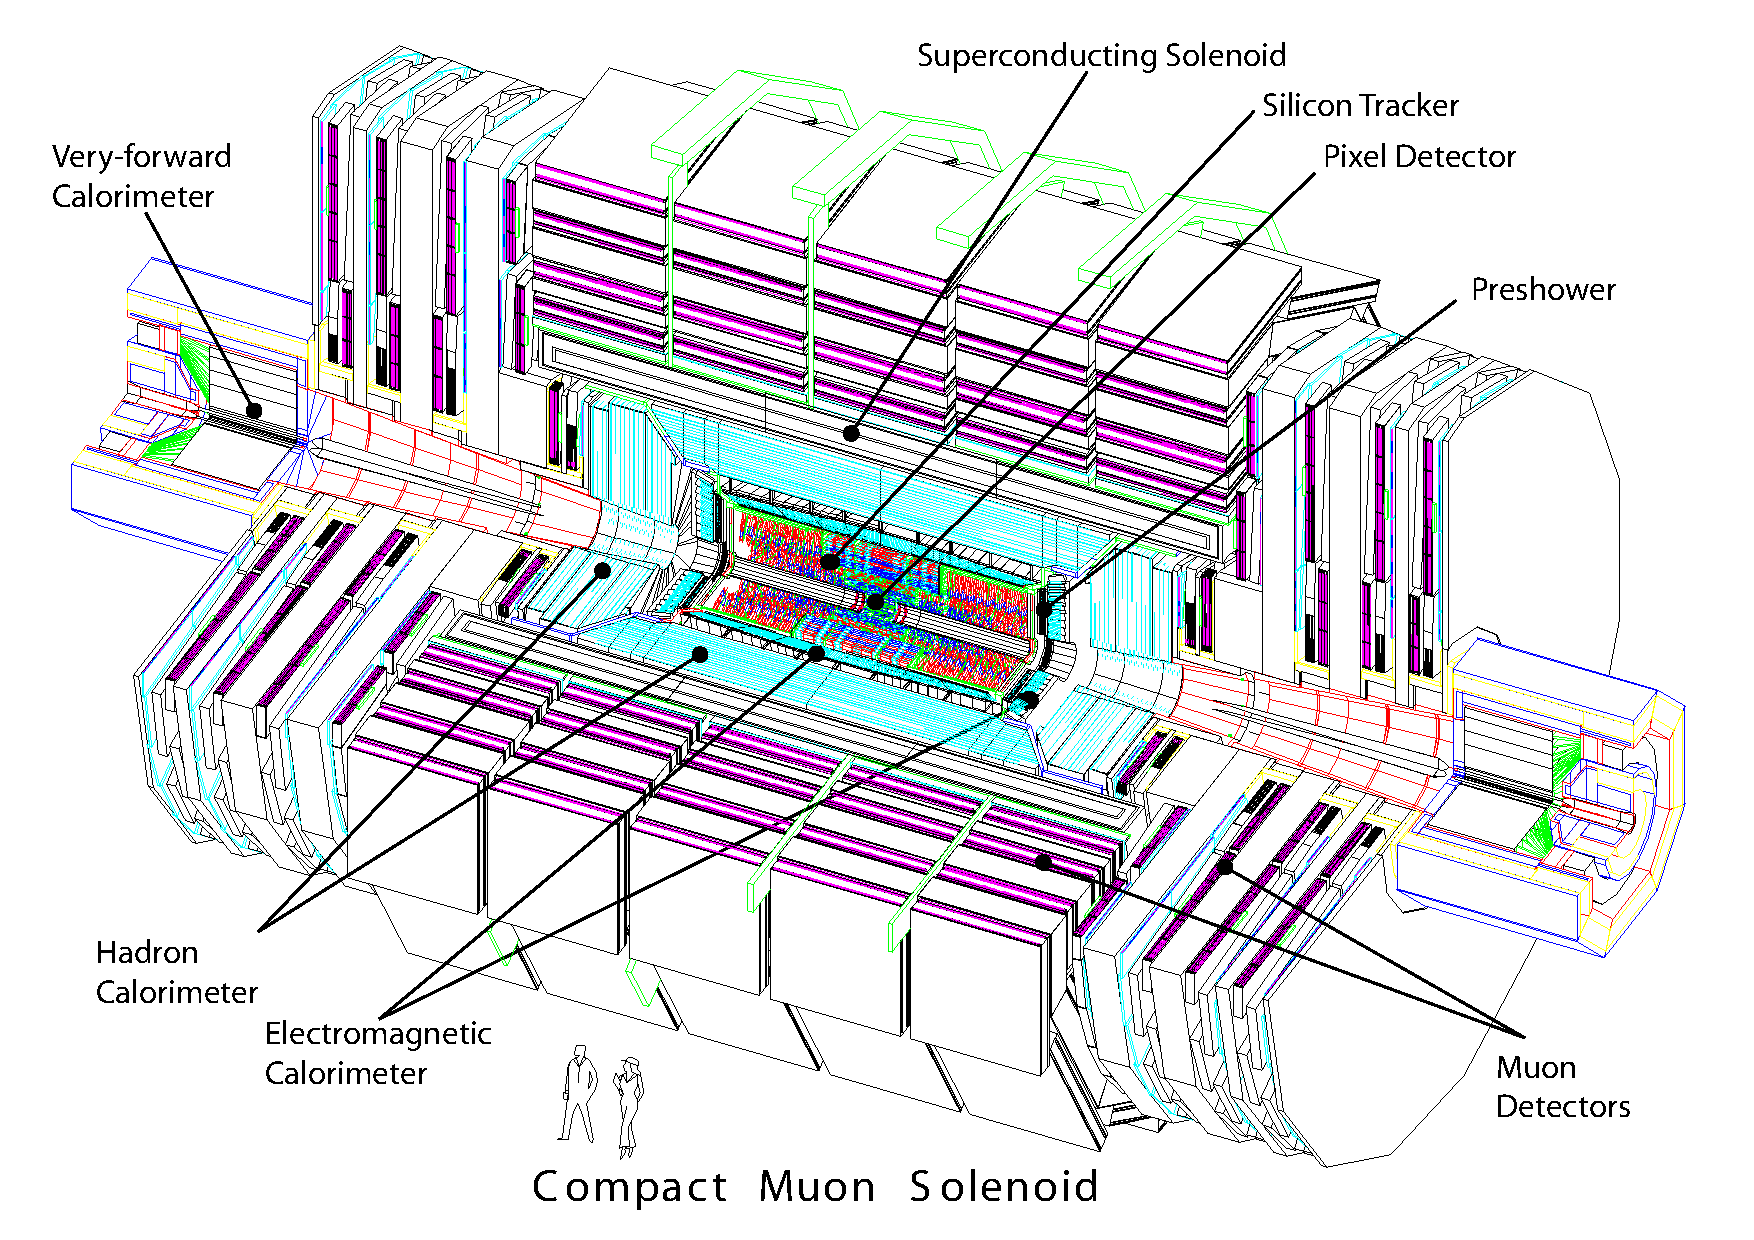
\includegraphics[width=0.95\textwidth]{figures/cms_complete_labelled.pdf}
\caption{The layout of the CMS detector, with the subdetectors labeled and two humans shown for a height reference.}
\label{fig:cms-overall}
\end{center}
\end{figure}

The center of the detector, the interaction point (IP), is used as the origin of the right-handed coordinate system that describes locations and directions within the detector. The $z$-axis is assigned to the direction of the LHC beam line, pointing anti-clockwise in the direction of Beam 2. The polar angle $\theta$ is defined as the angle away from the positive $z$-axis. This angle is often transformed into pseudorapidity, defined as $\eta = -\text{ln}[\text{tan}(\theta/2)]$, which has several desirable properties. It is independent of the particle mass and energy, and it is approximately equal to the rapidity for relativistic particles. Differences in pseudorapidity are Lorentz invariant for boosts in the $z$ direction, and particle production is approximately uniform in $\eta$.

The plane transverse to the $z$-axis comprises the $x$- and $y$-axes, with the $x$-axis pointing toward the center of the LHC ring and the $y$-axis pointing upward in the normal direction. The azimuthal angle $\phi$ is defined as the angle away from the positive $x$-axis in the transverse plane, and the radial coordinate $r$ is defined as the distance from the origin in the transverse plane. The magnitude of the component of momentum in the transverse plane is labeled \pt. The total transverse momentum of every event must be conserved, so the negative vector sum of \vecpt for all particles in the event is defined as the missing transverse momentum: $\vecmet = - \sum_{i} \vecpt^{(i)}$. The magnitude of this quantity is called the missing transverse energy, denoted as \met.

As a general purpose detector, the CMS experiment detects all long-lived SM particles, except neutrinos, which can only be measured by omission in the transverse plane via \met. These particles can be categorized as electrons, photons, muons, charged hadrons, and neutral hadrons. The latter two categories are usually found grouped into cones called jets, and can originate from gluons, light quarks, bottom quarks with displaced vertices, or hadronically decaying tau leptons. The identification of particles and related objects with the CMS detector is described in more detail in Ch. \ref{ch:reconstruction}.

The CMS detector must measure these particles with sufficient accuracy to accomplish the experiment's physics goals, imposing requirements which are met by the combination of the CMS subdetectors. The inner tracker measures event vertices and charged-particle momentum, with the help of the superconducting solenoid. The measurement of muon momentum is supplemented by the muon system. The electromagnetic calorimeter measures electron and photon energy, and the hadron calorimeter measures the energy from charged and neutral hadrons. In addition, the LHC operates at a high instantaneous luminosity, approaching $10^{34}\percms$; with an expected proton-proton cross section of 100\unit{mb} at the LHC center-of-mass energies, the collision rate is approximately 1\unit{MHz}. To cope with this incredibly high collision rate, the CMS experiment employs a trigger system to select interesting events at a rate slow enough to be stored and processed by the computing systems. The delivered luminosity is also measured by the detector, using several different techniques. The following sections describe the LHC, based on Ref. \cite{LHCmachine}, and the CMS subdetector systems, based on Ref. \cite{CMSJINST}.

\section{The Large Hadron Collider}

The Large Hadron Collider is the largest machine ever built and the highest-energy collider in the world. It uses the tunnel originally constructed for the Large Electron-Positron Collider (LEP) with a circumference of 26.7\unit{km}. The tunnel is located underground in Switzerland and France, near Geneva. Figure \ref{fig:lhc-diagram} shows a diagram of the LHC with the major experiments labeled. Opposite from CMS is A Toroidal LHC ApparatuS (ATLAS) at Point 1, the other general purpose detector. To the right of ATLAS at Point 8 is the LHC beauty (LHCb) experiment, which studies flavor physics. To the left of ATLAS at Point 2 is A Large Ion Collider Experiment (ALICE), which studies heavy ion physics in Pb-Pb and p-Pb collisions.

\begin{figure}[hbt]
\begin{center}
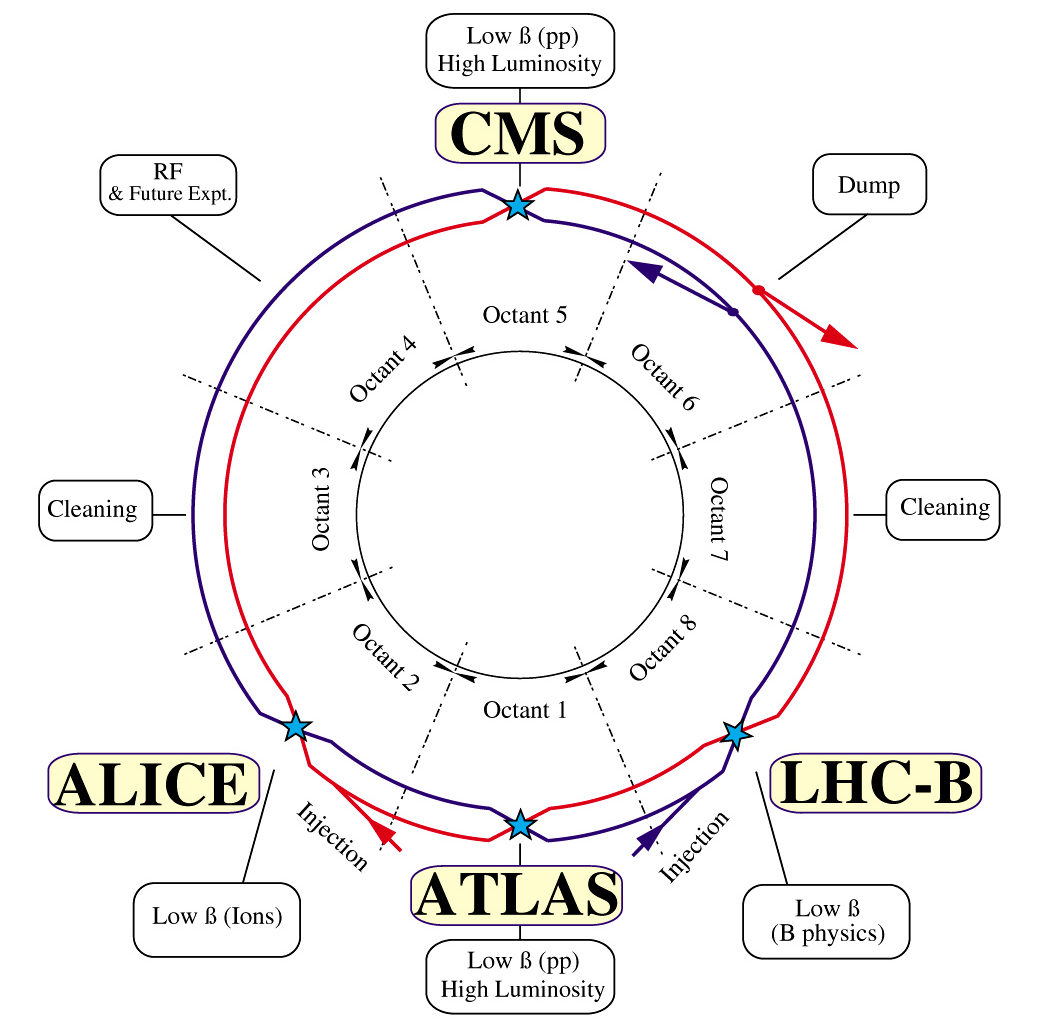
\includegraphics[width=0.95\textwidth]{figures/lhc-pho-1997-060.png}
\caption{A diagram of the LHC with the major experiments labeled \cite{Jean-Luc:841573}.}
\label{fig:lhc-diagram}
\end{center}
\end{figure}

The LHC is designed to accelerate two beams of protons up to energies of 7\TeV each, at instantaneous luminosities up to $10^{34}\percms$. It is also designed to accelerate lead ions up to energies of 1.38\TeV per nucleon, at instantaneous luminosities up to $10^{27}\percms$. The LHC can achieve energies several orders of magnitude higher than LEP in the same tunnel by using protons instead of electrons; the larger mass of protons reduces losses from synchrotron radiation by $(m_{\Pp}/m_{\Pe})^{4} = 1836^{4} = 1.136\times10^{13}$. The use of supercooled superconducting magnets, discussed below, is also crucial. Several stages of CERN accelerators are used to inject proton beams into the LHC, as shown in Fig. \ref{fig:lhc-injectors}. These include the linear accelerator Linac2, the Proton Synchrotron Booster (PSB), the Proton Synchrotron (PS), and the Super Proton Synchrotron (SPS). For lead ions, Linac3 and the Low Energy Ion Ring (LEIR), repurposed from the Low Energy Antiproton Ring (LEAR), are used instead of Linac2 and the PSB, respectively. The accelerated protons are grouped into bunches using radio frequency (RF) electromagnetic fields. The LHC is designed to accommodate a bunch spacing of 25\unit{ns}.

\begin{figure}[hbt]
\begin{center}
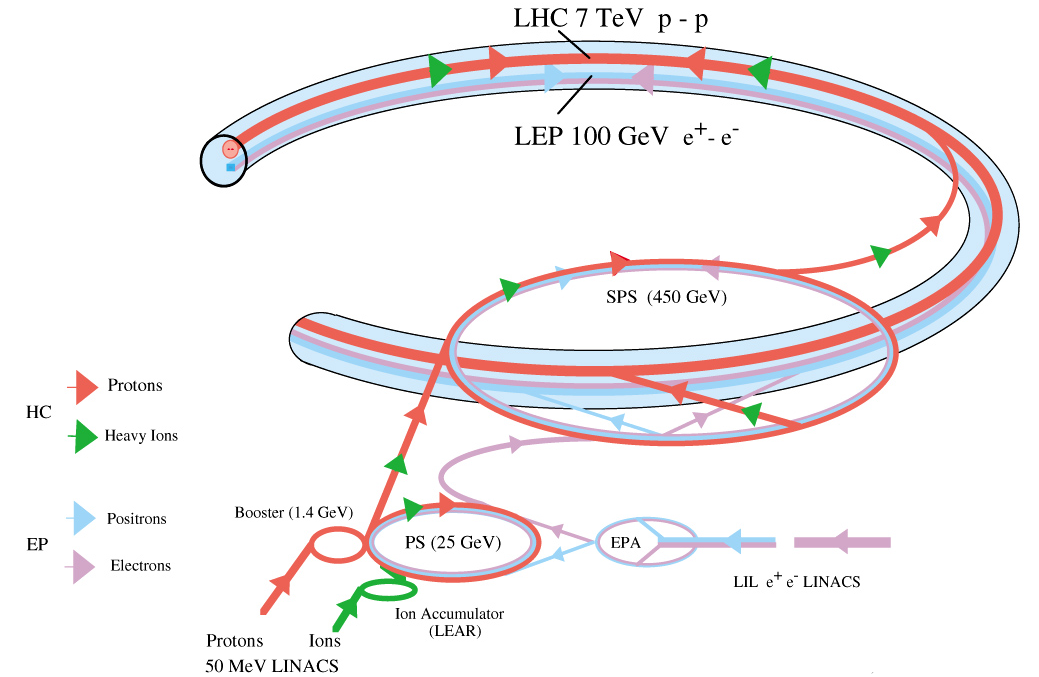
\includegraphics[width=0.95\textwidth]{figures/lhc-pho-1993-008.png}
\caption{A diagram of the CERN accelerators which form the LHC injector \cite{Jean-Luc:841568}.}
\label{fig:lhc-injectors}
\end{center}
\end{figure}

Due to size limitations in the tunnel, the two rings used to accelerate the two proton beams are formed by twin bore magnets. Each magnet has a single mechanical structure and cryostat, in which are placed two coils and two beam channels. The dipole magnet coils use superconducting NbTi Rutherford cables cooled to 1.9\unit{K}, as shown in Fig. \ref{fig:lhc-dipole}, with a design field strength of 8.33\unit{T} for acceleration of protons up to 7\TeV. This extreme cooling is accomplished using superfluid helium. In total, the LHC contains 1232 dipole magnets. Thousands of quadrupole, sextupole, octupole, and decapole magnets are used to correct and focus the beam.

\begin{figure}[hbt]
\begin{center}
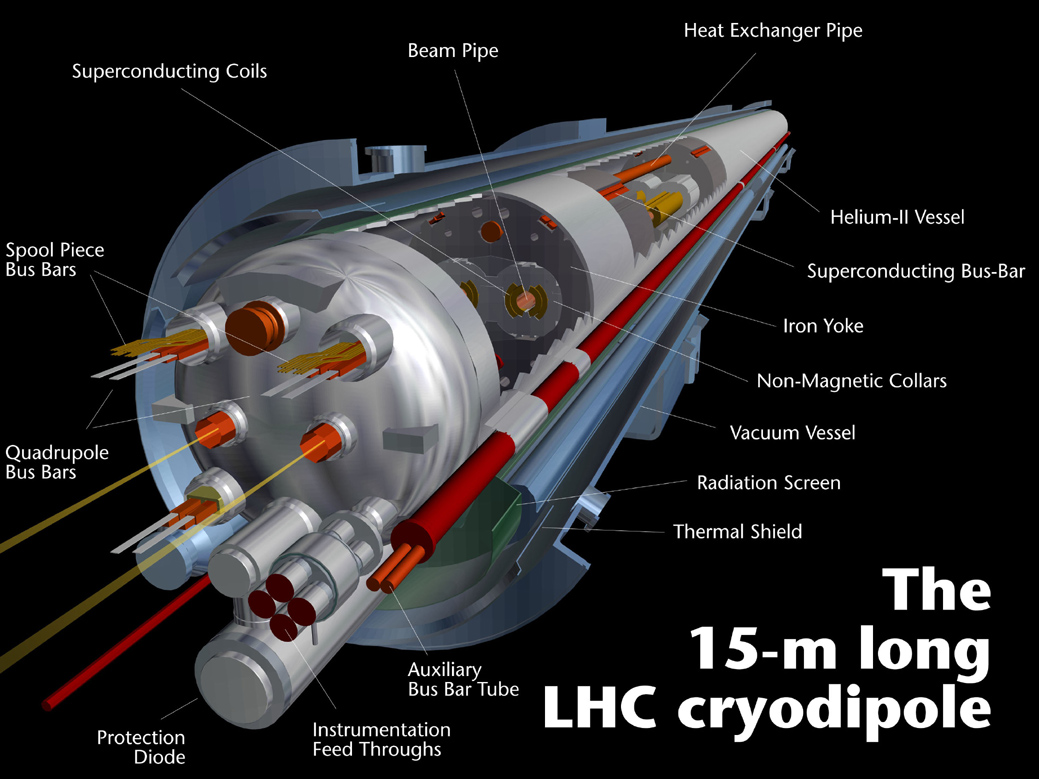
\includegraphics[width=0.95\textwidth]{figures/lhc-pho-1998-299.jpg}
\caption{A diagram of an LHC dipole magnet, with the major components labeled \cite{Dailler:842253}.}
\label{fig:lhc-dipole}
\end{center}
\end{figure}

In 2012, the LHC accelerated proton beams to energies of 4\TeV each, with a peak instantaneous luminosity of $7.67\times10^{33}\percms$ and a bunch spacing of 50\unit{ns}. During that year, it delivered 23.30\fbinv of integrated luminosity to the CMS detector, of which 21.79\fbinv was recorded \cite{LumiPublic}. In the upcoming 2015 run, the LHC will achieve its design energy, instantaneous luminosity, and bunch spacing.

\section{Tracker}
\label{sec:tracker}

The CMS tracker is the first subdetector to measure charged particles produced in collisions at the IP. It is 5.8\unit{m} long and 2.5\unit{m} in diameter, covering the pseudorapidity range $-2.5 < \eta < 2.5$. Two subsystems make up the tracker: the pixel detector and the silicon strip tracker. The layout of the tracker, with these subsystems labeled, is shown in Fig. \ref{fig:tk-layout}. Due to the tracker's location close to the IP, it experiences severe radiation doses that are expected to range from 0.18 to 84\unit{Mrad} after 500\fbinv of data. Hence, the tracker must be robust against radiation damage, requiring operation at $-10\degC$ and influencing the design of the sensors and electronics. For tracks with momentum of 100\GeV, the tracker has a transverse momentum resolution of 1--2\% for $|\eta|<1.6$; at higher $\eta$, the reduced transverse depth of the tracker degrades the resolution.

\begin{figure}[hbt]
\begin{center}
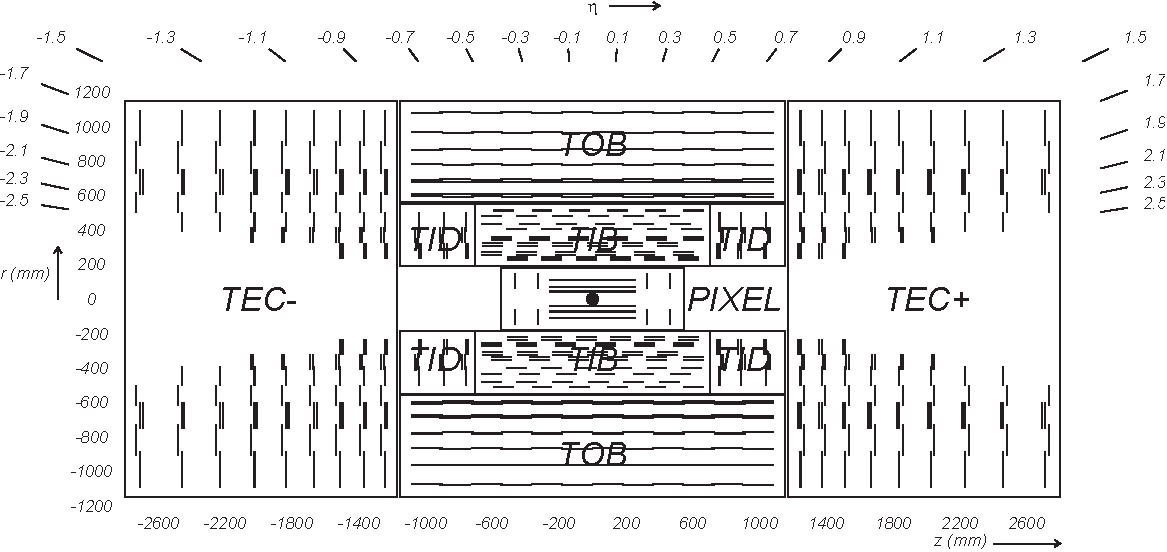
\includegraphics[width=0.95\textwidth]{figures/CMS_tracker.pdf}
\caption{The layout of the CMS tracker, with subsystems labeled.}
\label{fig:tk-layout}
\end{center}
\end{figure}

The pixel detector is the innermost portion of the tracker. It consists of three barrel layers, collectively called BPIX, and two endcap layers, called FPIX. Each pixel cell is a hybrid silicon detector with dimensions $100\times150\mum^{2}$. The small pixel size enables precise track resolutions of 10\mum in the $r$-$\phi$ direction and 20\mum in the $z$ direction. In total, the BPIX comprises 48 million pixels and the FPIX comprises 18 million pixels. The pixel detector is important for many key components of CMS physics analysis. These include the reconstruction of secondary vertices from decays of tau leptons and bottom quarks, as well as producing seed tracks for the strip tracker and the high level trigger.

The silicon strip detector consists of four subsystems. The Tracker Inner Barrel (TIB) has four layers with the three-layer Tracker Inner Disks (TID) at each end; both systems' strips are 320\mum thick. Surrounding the TIB/TID is the Tracker Outer Barrel (TOB), which has six layers. The first four layers of the TOB use 500\mum thick strips, while the last two layers use 122\mum thick strips. The Tracker EndCaps (TEC) have nine disks with up to seven layers of strips, 320\mum thick in the inner four rings and 500\mum thick in the outer three rings. In total, all of these layers contain 9.3 million silicon strips.

The tracker maintained excellent performance during the 2012 run of the LHC. The pixel detector had 97.7\% of channels operational in BPIX and 92.8\% of channels operational in FPIX, while 97.5\% of channels in the strip detector were active. The hit reconstruction efficiencies were greater than 99\% for each layer of the strip detector and greater than 99.5\% for each layer of the pixel except for the first layer of BPIX, which had an efficiency greater than 99.2\% \cite{Veszpremi:2014hpa}. 

\section{Electromagnetic Calorimeter}

The electromagnetic calorimeter (ECAL) is a homogeneous calorimeter constructed entirely of lead tungstate (\pbwo) crystals. The ECAL is divided into two subsystems: the ECAL barrel (EB) and the ECAL endcap (EE). In the endcap region, there is an additional ECAL preshower (ES) detector in front of the EE. Figure \ref{fig:ecal-layout} displays these subsystems. \pbwo has a peak emission wavelength of 425\unit{nm} and many desirable material properties. These properties include high density ($8.28\unit{g/cm}^3$), short radiation length (0.89\cm), short Moli\`{e}re radius (2.2\cm), and fast decay time (6\unit{ns}). The use of homogeneous \pbwo crystals enables precise energy resolution for electromagnetic objects. For photons with $\ET \approx 60\GeV$, the energy resolution ranges from 1.1\% to 2.6\% for the EB and 2.2\% to 5.0\% for the EE. In general, the energy resolution $\sigma$ varies as a function of energy $E$ in \GeVns:
\begin{equation}
\label{eq:ecal-res} \left(\frac{\sigma}{E}\right)^{2} = \left(\frac{S}{\sqrt{E}}\right)^{2} + \left(\frac{N}{E}\right)^{2} + C^{2}.
\end{equation}
In Eq. \eqref{eq:ecal-res}, $S$ is the stochastic term, $N$ is the noise term, and $C$ is the constant term. Typical values for these terms were measured by a test beam to be $S=2.8\%$, $N=12\%$, $C=0.30\%$.

\begin{figure}[hbt]
\begin{center}
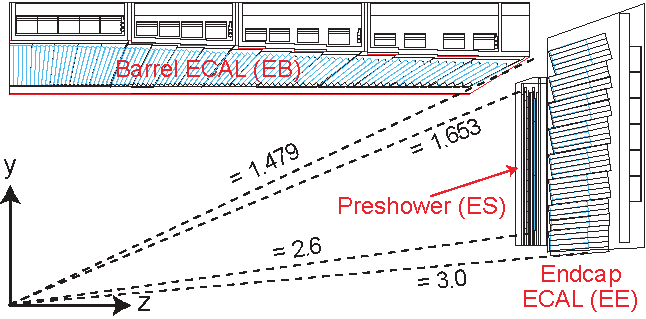
\includegraphics[width=0.95\textwidth]{figures/ECAL_transverse_section.pdf}
\caption{A diagram of the CMS ECAL, with subsystems and $\eta$ ranges labeled.}
\label{fig:ecal-layout}
\end{center}
\end{figure}

The EB contains 61200 \pbwo crystals and covers the range $|\eta|<1.479$. The crystals are arranged in a projective geometry with a tapered shape. The crystal granularity is approximately $0.0174\times0.0174$ in $\eta$-$\phi$, corresponding to dimensions of $22\times22\mm^{2}$ at the front face and $26\times26\mm^{2}$ at the back face. The EB has a depth of 230\mm or 25.8 radiation lengths ($X_{0}$). The scintillation light produced by the \pbwo crystals is read out using avalanche photodiodes (APDs). At 18\degC, the APDs measure approximately 4.5 photoelectrons per \MeVns. The dark current of the APDs is sensitive to radiation exposure. Over the course of the 2012 run, the dark current ranged from 0.3--1.3\muA on average, corresponding to an average noise of 47--57\MeV \cite{CMS:2013ecal}.

The EE contains 14648 \pbwo crystals and covers the range $1.479<|\eta|<3.0$. The crystals are arranged in a non-projective $x$-$y$ geometry, with dimensions of $28.62\times28.62\mm^{2}$ at the front face and $30\times30\mm^{2}$ at the back face. The EE has a depth of 220\mm or 24.7$\,X_{0}$. Vacuum phototriodes (VPTs) are used as the photodetectors to read out the scintillation light from the \pbwo crystals. They collect approximately 4.5 photoelectrons per \MeVns at 18\degC. During the 2012 run, the average noise ranged from 180--220\MeV, with a more dramatic increase up to 600\MeV at high $\eta$ because of the high radiation dose \cite{CMS:2013ecal}.

The ES is intended to identify neutral pions in the endcap region, covering the range $1.653<|\eta|<2.6$. It is a sampling calorimeter with two layers of lead absorber and silicon strip detectors. The first layer of lead absorber has a thickness of 2$\,X_{0}$, while the second layer has a thickness of 1$\,X_{0}$. Each layer of silicon strips is 320\mum thick and can collect 3.6\unit{fC} of charge from a minimum ionizing particle.

%add percentage of live channels for EB and EE in 2012 run? and HE raddam?

\section{Hadron Calorimeter}

The hadron calorimeter (HCAL) is a sampling calorimeter which measures the energy of hadronic particles. The HCAL is especially important for measuring neutral hadrons, which do not leave tracks in the tracker. In addition, by containing all hadronic activity in each event within $|n|<5$, the HCAL enables the measurement of \met caused by neutrinos and other theoretical weakly-interacting particles. The HCAL consists of four subsystems. Three of these subsystems use similar technology: the HCAL barrel (HB), the HCAL endcap (HE), and the HCAL outer (HO). The fourth subsystem, the HCAL forward (HF), uses an alternative technology necessary to survive the high radiation doses at its forward location. The locations of the various HCAL subsystems in the CMS detector are shown in Fig. \ref{fig:hcal-layout}. The calorimeter system, combining the ECAL and the HCAL, can measure jets with a resolution $\sigma/E \approx 100\% / \sqrt{E\,[\GeVns]} \oplus 5\%$ that varies with the jet energy $E$.

\begin{figure}[hbt]
\begin{center}
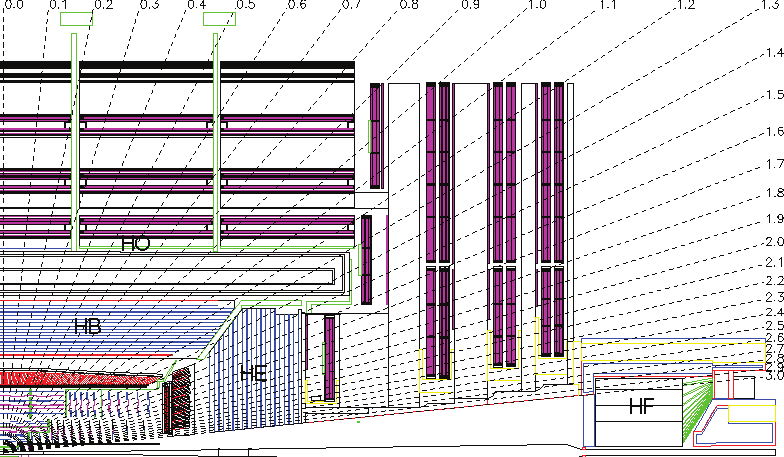
\includegraphics[width=0.95\textwidth]{figures/HCAL_subdet.pdf}
\caption{The layout of the HCAL subsystems HB, HE, HO, and HF in the CMS detector.}
\label{fig:hcal-layout}
\end{center}
\end{figure}

The HB is a 16-layer sampling calorimeter covering the range $|\eta|<1.3$. The absorbing layers are made of C26000 cartridge brass, composed of 70\% copper and 30\% zinc. Cartridge brass has a density of $8.53\unit{g/cm}^3$, a radiation length of 1.49\cm, and a nuclear interaction length of 16.42\cm. The first absorbing layer in the HB is a 40-mm-thick steel plate. The next eight absorbing layers are 50.5-mm-thick brass plates, and the subsequent six absorbing layers are 56.5-mm-thick brass plates. The last absorbing layer is a 75-mm-thick steel plate. The overall thickness of the HB absorber ranges from 5.82$\,\lambda_{0}$ at $\eta=0$ to 10.6$\,\lambda_{0}$ at $|\eta|=1.3$. The EB in front of the HB has a thickness of 1.1$\,\lambda_{0}$ and can measure the electromagnetic portions of early developing hadronic showers. The scintillating layers consist of 3.7-mm-thick Kuraray SCSN81 plastic scintillator, a polystyrene base doped with fluors. The exception is Layer 16, which has a thickness of 9\mm, in order to sample more from late developing hadronic showers. At the front of the HB, before the first absorbing layer, is the scintillator Layer 0, which is 9\mm of Bicron BC408 plastic scintillator, a polyvinyltoluene base doped with fluors. Layer 0 samples the energy deposited by hadronic showers in the dead material between the EB and the HB. The scintillator tiles are arranged in a projective geometry with a granularity of $0.087\times0.087$ in $\eta$-$\phi$. In total, the HB has 16 $\eta$ divisions called towers, 36 $\phi$ divisions, and approximately 70000 tiles. The light from the scintillators is collected by Kuraray Y-11 green wavelength shifting (WLS) fiber, which is placed in a $\sigma$-shaped groove in the scintillator tiles. The wavelength-shifted light from multiple layers is brought together and read out by hybrid photodiodes (HPDs). These photodetectors were chosen because of their large dynamical range and low sensitivity to magnetic fields.

The thinness of the HB at low $\eta$ prevents it from fully containing hadronic showers, so the HO is added to act as an extension of the calorimeter system. The HO uses the same scintillator tile technology as the HB: 3.7-mm-thick SCSN81 with Y-11 WLS fiber and granularity $0.087\times0.087$ in $\eta$-$\phi$, read out by HPDs. The HO is divided into five rings, each with a width of 2.536\unit{m} in the $z$ direction, based on the structure of the iron return yoke outside of the solenoid. In the central Ring 0, the HO has two scintillating layers, one inside the solenoid and one outside of it. In the other rings, the HO has one scintillating layer outside of the solenoid. The thickness of the absorbing iron layer formed by the solenoid is 19.5\cm, extending the total depth of the calorimeter system to a minimum of 11.8$\,\lambda_{0}$.

The HE is a 17-layer sampling calorimeter covering the range $1.3<|\eta|<3.0$. Each absorbing layer consists of 79-mm-thick cartridge brass, the same material used for the HB absorbing layers. The scintillating layers use the same technology as the HB and the HO. In total, the HE contains 20916 scintillator tiles. The granularity of the tiles is the same as HB for $|eta|<1.6$; for higher $\eta$, they become coarser at approximately $0.17\times0.17$ in $\eta$-$\phi$. Unlike the HB, the scintillating layers in each tower are split into multiple groups called depths before being read out by HPDs. A diagram of the depth segmentation scheme is shown in Fig. \ref{fig:hcal-depths}. This depth segmentation allows for more precise recalibration of the HE, which experiences a higher radiation dose than the HB. Towers 27, 28, and 29, which are the closest to the beamline, have three readout depths, while the other towers have two readout depths. The crossover region between the HB and the HE, towers 15 and 16, also utilize depth segmentation. As in the HB, Layer 0 in the HE consists of 9-mm-thick BC408 to sample from the dead material between the EE and the HE. The combined calorimeter system, including both the EE and the HE, has an approximate thickness of 10$\,\lambda_{0}$.

The HF covers the range $3.0<|\eta|<5.0$, with no ECAL in front of it. It consists of a steel absorber structure with a thickness of 165\cm or 10$\,\lambda_{0}$. Polymer-cladded quartz fibers with diameter 800\mum are embedded in the steel absorber. The fibers are bundled together to form 13 towers in a non-projective $x$-$y$ geometry with granularity $0.175\times0.175$ in $\eta$-$\phi$. Over 1000\unit{km} of fiber is used in the HF. Half of the fibers run for the full 165\cm depth of the detector, while the other half start 22\cm into the detector. Each type of fiber is read out separately in order to distinguish electromagnetic showers from hadronic showers. The fibers measure particle showers using Cherenkov light, which is read out by photomultiplier tubes (PMTs). They measure approximately 1 photoelectron for every 4\GeV of energy deposited. This alternative design was necessary to ensure the radiation hardness of the HF, parts of which can experience 100\unit{Mrad/year}.

\begin{figure}[hbt]
\begin{center}
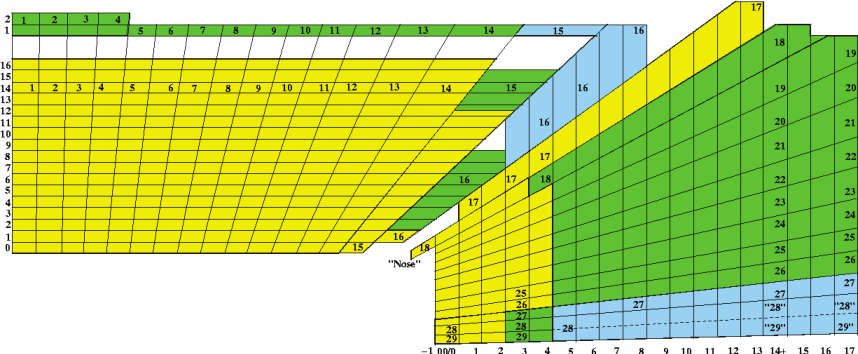
\includegraphics[width=0.95\textwidth]{figures/HCAL_tower_segmentation.pdf}
\caption{A diagram of the depth segmentation scheme in the HB and the HE.}
\label{fig:hcal-depths}
\end{center}
\end{figure}

%add percentage of live channels for HCAL in 2012 run?

\section{Solenoid}

The superconducting solenoid is the central feature of the CMS detector. The solenoid provides a magnetic field of 3.8\unit{T} within the volume formed by its diameter of 6\unit{m} and length of 12.5\unit{m}. This strong magnet field is necessary so that high energy charged particles bend sufficiently for the tracker to measure their momenta accurately. At full current, the solenoid has a stored energy of 2.35\unit{GJ}. The magnet is constructed from a 4-layer winding of reinforced NbTi conductor, cooled to 4.5\unit{K}. It is split into five rings of equal length. The cold mass of the magnet is 220 tons, and the high ratio between the stored energy and the cold mass, 11.6\unit{KJ/kg}, causes a significant mechanical deformation of 0.15\% when the magnet is powered. Figure \ref{fig:solenoid} shows an artistic rendering of the solenoid.

\begin{figure}[hbt]
\begin{center}
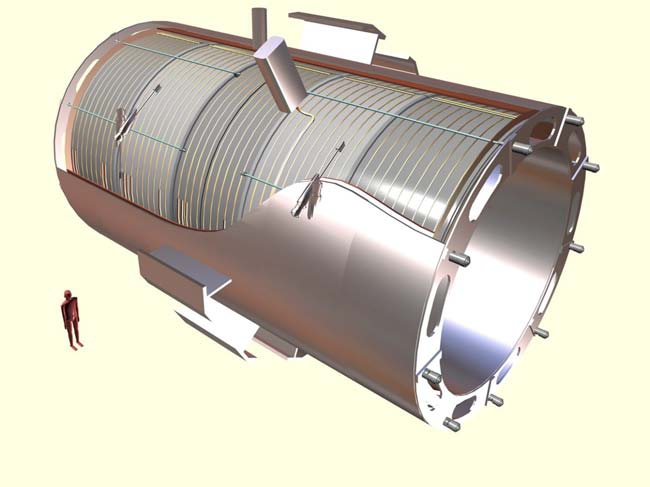
\includegraphics[width=0.95\textwidth]{figures/CMS_solenoid.jpg}
\caption{An artistic rendering of the CMS solenoid, showing the five rings placed inside the cryostat, along with the support structure.}
\label{fig:solenoid}
\end{center}
\end{figure}

\section{Muon System}
\label{sec:muon-system}

The identification and measurement of muons is a major focus of the CMS experiment. The CMS muon system comprises three subsystems, each utilizing different gaseous particle detection technology. In the barrel region, drift tubes (DTs) are used. In the endcap region, cathode strip chambers (CSCs) are used. Resistive plate chambers (RPCs) are also used in both regions. The muon systems are built into the iron yoke, which consists of five barrel rings and six endcap disks weighing 10000 tons in total. The yoke confines the outer magnetic field from the return flux from the solenoid and absorbs stray hadrons. The layout of the muon system is shown in Fig. \ref{fig:muon-system}. The momentum resolution of the muon system by itself is approximately 9\% for $\pt<200\GeV$ with low $\eta$ and low $p$. For 1\TeV muons, the resolution varies between 15\% and 40\%, depending on $|\eta|$. When the muon system measurements are combined with measurements from the tracker, the 1\TeV muon resolution is improved to 5\%.

\begin{figure}[hbt]
\begin{center}
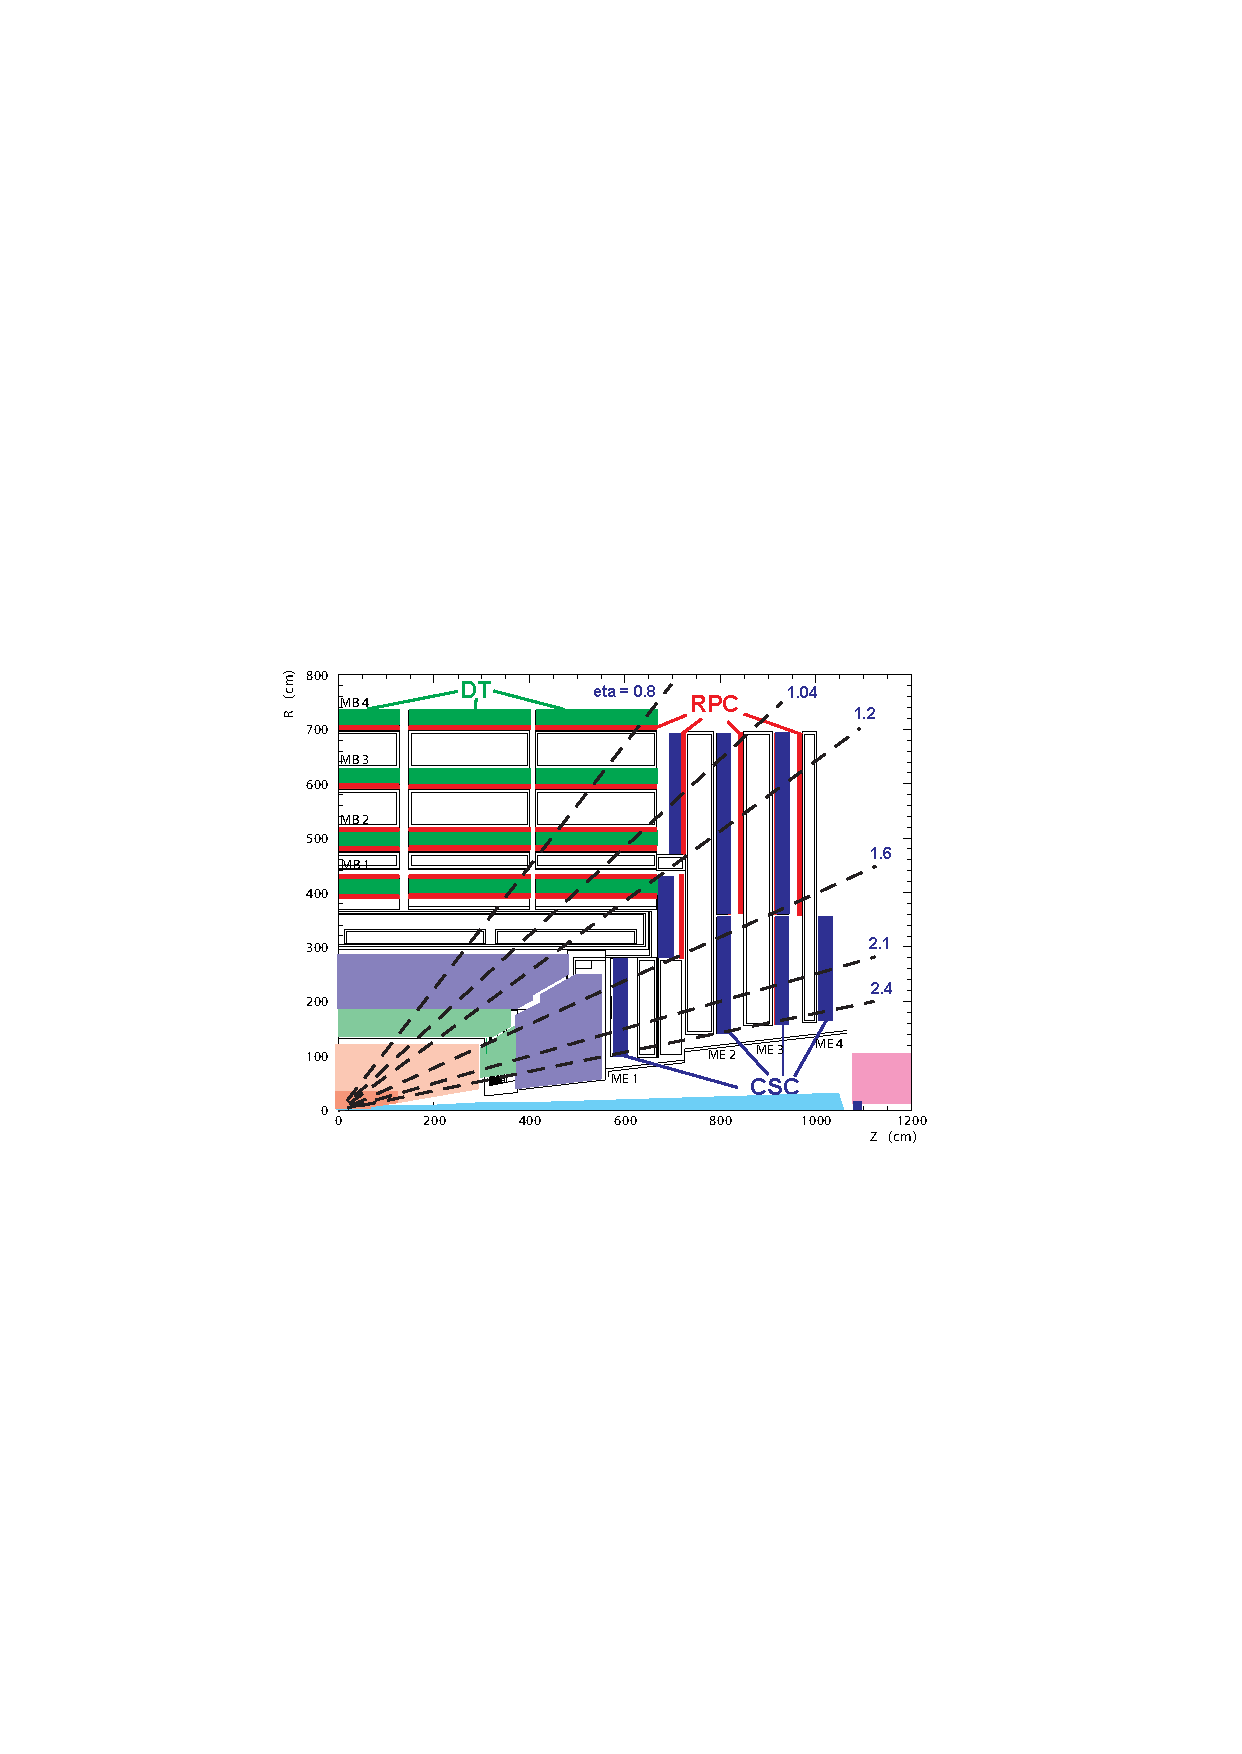
\includegraphics[width=0.95\textwidth]{figures/CMS_muon_system.pdf}
\caption{The layout of the muon system, with the three subsystems labeled.}
\label{fig:muon-system}
\end{center}
\end{figure}

The DTs are divided into four stations, which together cover the range $|\eta|<1.2$ and are labeled MB1 through MB4 (Muon Barrel). The first three stations each contain twelve chambers divided into three groups of four. Two of the groups of four measure the $r$-$\phi$ coordinate of muons, while the third group of four measures the $z$ coordinate. MB4 does not include a group of chambers that measures $z$. All four stations together contain 250 DTs with a total of 172000 sensitive wires. The gas used in the DTs is a mixture of 85\% Ar and 15\% $\text{CO}_2$, and the anode wires are gold-plated stainless steel with a diameter of 50\mum. Within $|\eta|<0.8$, the MB stations alone can reconstruct high-\pt muon tracks with an efficiency exceeding 95\%. The global $r$-$\phi$ resolution is 100\mum.

The CSCs are also divided into four stations and cover the range $0.9<|\eta|<2.4$. The four stations are labeled ME1 through ME4 (Muon Endcap). Each station is divided into several groups as follows: ME1 has three groups of 72 CSCs; ME2 and ME3 each have one group of 36 CSCs and another group of 72 CSCs; ME4 has one group of 36 CSCs. The total number of CSCs is thus 468. The cathode strips are arranged in the radial direction to measure the $r$-$\phi$ coordinate, while the anode wires are perpendicular to the strips to measure $\eta$. There are approximately 220000 cathode strip readout channels and 180000 anode wire readout channels. The CSC gas mixture is set at 40\% AR, 50\% $\text{CO}_2$, and 10\% $\text{CF}_4$. The cathode strips are formed from a fiberglass/epoxy material called FR4, coated with 36-$\mu$m-thick copper. The anode wires are made of gold-plated tungsten with a diameter of 50\mum. The first group of ME1 CSCs uses slightly thinner wire with 30\mum diameter and has some other slightly modified properties.

To complement the DTs and CSCs, RPCs are installed in both the barrel and endcap regions, covering the range $|\eta|<1.6$. The RPCs are primarily used to provide muon trigger information, due to fast tagging capabilities which allow them to precisely identify the bunch crossing time of muon candidate events. MB1 and MB2 each have one internal and one external group of RPCs, relative to the DTs; MB3 and MB4 each have two internal groups of RPCs. These groups together comprise 480 chambers. In the endcap, there are three RPC stations mounted in concentric circles on the iron yoke disks, with a total of 144 chambers. The RPCs are parallel plate detectors filled with a gas mixture of 96.2\% $\text{C}_2\text{H}_2\text{F}_4$, 3.5\% $i\text{C}_4\text{H}_{10}$, and 0.3\% $\text{SF}_6$.

%add percentage of live channels for muon system in 2012 run?

\section{Trigger}

The CMS trigger is necessary to reduce the roughly 1\unit{MHz} rate of collision events produced by the LHC to a rate which can be stored and processed. The trigger system consists of two stages. The first stage uses hardware and is called the Level-1 (L1) Trigger. The L1 Trigger is designed to have a maximum output rate of 100\unit{kHz}. The second stage is the High Level Trigger (HLT), which uses software and reduces the output rate to $\mathcal{O}(100\unit{Hz})$.

The L1 Trigger uses custom-built programmable electronics, including field-programmable gate arrays (FPGAs), application-specific integrated circuits (ASICs), and memory lookup tables (LUTs). All of the subdetectors send input to the L1 Trigger, which is organized into local, regional, and global components as shown in Fig. \ref{fig:L1-trigger}. The local components, Trigger Primitive Generators (TPGs), are constructed from energy deposits in the calorimeters and track segments or hit patters from the muon system.

The TPGs from the ECAL, the HCAL, and the HF are combined into the Regional Calorimeter Trigger (RCT). The RCT groups calorimeter trigger towers into regions, which are made up of four towers in the barrel and endcap, and one tower in the HF. These regions are used to determine electron and photon candidates, as well as transverse energy sums (\sumet) and tau-jet vetoes. The RCT also passes MIP and isolation information to the muon triggers. Using information from the RCT, the Global Calorimeter Trigger (GCT) determines jet candidates and counts, providing up to four jets and four tau-jets from the central HCAL and four jets from the HF. The GCT also determines total \ET, \met, and \HT, which is calculated as \sumet for all jets above a certain threshold.

In parallel, the muon DT, CSC, and RPC systems each produce their own local triggers. The Regional Muon Trigger (RMT) contains the DT and CSC Track Finders (DTTF, CSCTF) which make tracks using segments from their respective subdetectors. As mentioned in Sec. \ref{sec:muon-system}, the RPCs act as a dedicated trigger using their timing resolution of 1\unit{ns} to determine bunch crossing times. The Global Muon Trigger (GMT) combines the information from the RMT and RPCs to produce up to four muon candidates in each of the barrel and endcap regions. These candidates include the following information: \pt, charge, $\eta$, $\phi$, a quality code, MIP, and isolation.

Finally, the Global Trigger (GT) combines the GCT and GMT candidates and quantities to decide whether or not to keep the event, based on a set of L1 triggers with different criteria. The GT also uses information from the Trigger Control System (TCS) regarding the status of the subdetector readout and data acquisition systems. The Timing, Trigger, and Control (TTC) system is used to return the GT decision, called the Level-1 Accept (L1A), to the various subdetectors. This entire process is completed within 3.2\mus.

\begin{figure}[hbt]
\begin{center}
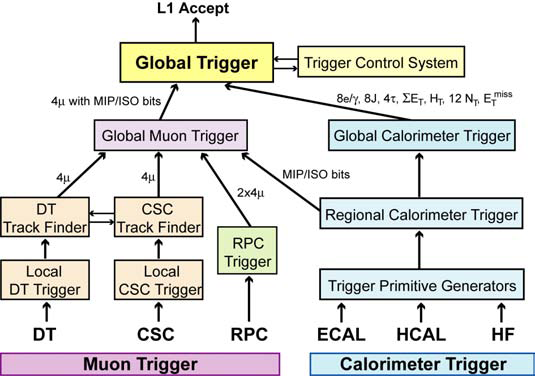
\includegraphics[width=0.95\textwidth]{figures/L1_architecture.png}
\caption{The architecture of the L1 Trigger.}
\label{fig:L1-trigger}
\end{center}
\end{figure}

The HLT further analyzes events which pass the L1A decision. Using a farm of roughly 1000 commercial processors comprised of over 13000 central processing units (CPUs), it approximately emulates the full offline reconstruction algorithms described in Ch. \ref{ch:reconstruction}. Like the L1 Trigger, the HLT uses a set of triggers with different criteria, called the trigger menu. Different trigger menus are constructed for various conditions, including different instantaneous luminosity levels and different types of collisions or measurements. The selected menu can be changed during the operation of the detector in response to new conditions. Events which pass the HLT decision are sorted into primary datasets (PDs) with minimal overlap. The HLT output includes several streams, including monitoring and calibration streams in addition to the primary stream of physics events.

During the 2012 run, the L1 Trigger operated at rates up to 100\unit{kHz} with only 3\% dead time \cite{Brooke:2013hnf}. The HLT operated at rates up to 1\unit{kHz} and took an average of 200\unit{ms} to process an event \cite{Trocino:2014jya}. This processing speed is two orders of magnitude faster than the full offline reconstruction. Around 600\unit{Hz} of HLT output data was ``parked'', or recorded to disk in a raw format before being processed. This data parking scheme took advantage of the impending 2013-2014 long shutdown for collider and detector upgrades, when CPUs would be available to process the extra data. The parked data was collected using alternative trigger menus designed to enable precision measurements and new physics searches in unexplored kinematic regions. CMS also engaged in ``data scouting'', performing simple analyses on partially-reconstructed events, for example keeping only HLT-reconstructed jets, from processes which would normally have rates too high to be accepted by the trigger. These simple analyses searched for noticeable deviations from SM predictions in order to indicate possible advantageous changes to the trigger menus.

\section{Luminosity Measurement}

The fine resolution of the CMS pixel detector (Sec. \ref{sec:tracker}) implies that a given pixel will tend to be activated by one track at most per bunch crossing. A minimum bias interaction creates an average of 200 clusters, with each cluster containing an average of 5 pixels \cite{CMS-PAS-LUM-12-001}. Even with 100 pileup events per bunch crossing, the pixel detector will have an occupancy as low as 0.1\%. The number of pixel hits should thus scale linearly with the number of interactions per bunch crossing for instantaneous luminosities up to and even beyond the LHC design performance. Equation \eqref{eq:pixel-lumi} shows how the instantaneous luminosity $\mathcal{L}$ is related to the average number of pixel clusters per event $\langle n \rangle$ \cite{CMS-PAS-LUM-13-001}:
\begin{equation} \label{eq:pixel-lumi}
\mathcal{L} = \frac{\nu \langle n \rangle}{\sigma_\text{vis}}.
\end{equation}
Here, $\nu = 11246\unit{Hz}$ is the LHC revolution frequency, $\langle n \rangle$ is defined as $\mu n_{1}$ where $\mu$ is the number of collisions per bunch crossing and $n_{1}$ is the average number of clusters per collision, and the visible cross section $\sigma_\text{vis}$ is defined as $\sigma_\text{T} n_{1}$ where $\sigma_\text{T}$ is the total inelastic cross section. A Van der Meer scan is used to calibrate $\sigma_\text{vis}$. In 2012, CMS measured the total integrated luminosity with a systematic uncertainty of 2.6\% using this method.

The HF is used as a second method of measuring the luminosity. This is possible because the HF can be run safely during unstable beams \cite{CMS-PAS-LUM-13-001}. Information from the HF can be used to measure the luminosity in two different ways. The average fraction of empty towers can be related to the mean number of interactions per crossing, or the average transverse energy per tower can be linearly related to the luminosity. It can make an online determination of the average luminosity to a statistical uncertainty of 1\% in under 1\unit{s}. However, the calibration of this measurement can drift over long time periods due to changes in the gain of the HF PMTs. In practice, the increase in pileup interactions observed during the 2012 run moves the HF response into a nonlinear regime, limiting the accuracy of this method. Because of these limitations, the HF method is utilized primarily as a cross-check for the pixel cluster counting method.
% input: [reconstruction.tex]
\chapter{Event Reconstruction
\label{ch:reconstruction}}

Particles created in proton-proton collisions pass through the CMS detector and leave signals in different subdetectors. Figure \ref{fig:cms-slice} shows examples of typical signals for different types of particles. Each type of particle has a different characteristic signature from which it can be identified using information from the various subdetectors. Muons, electrons, and charged hadrons create tracks in the tracker, while photons and neutral hadrons do not. Muons also create hits in the muon systems. Electrons and photons deposit energy in the ECAL, while charged and neutral hadrons deposit most of their energy in the HCAL.

\begin{figure}[hbt]
\begin{center}
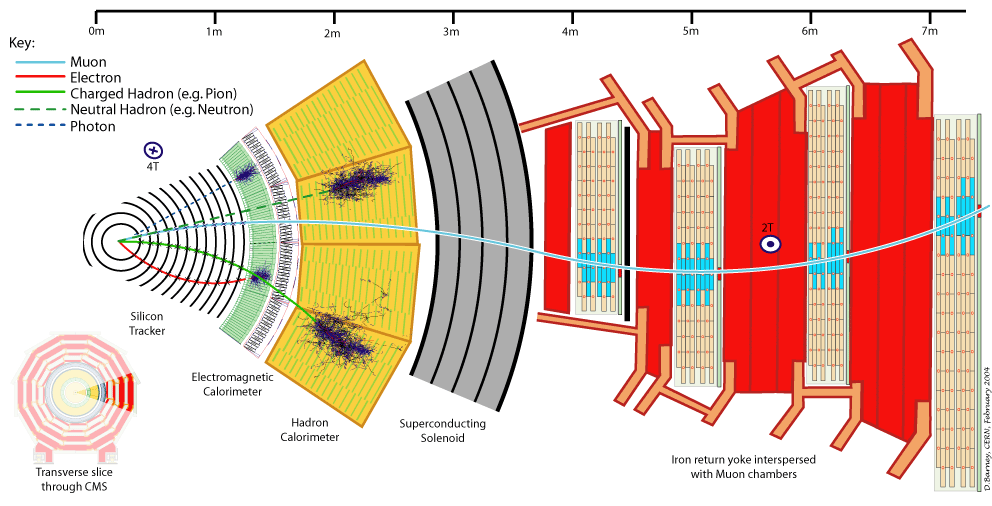
\includegraphics[width=0.95\textwidth]{figures/CMS_slice.png}
\caption{A cross-sectional view of the CMS detector with all subdetectors labeled and examples of signals left by muons, electrons, charged hadrons, neutral hadrons, and photons \cite{CMS-slice}.}
\label{fig:cms-slice}
\end{center}
\end{figure}

The raw output from each subdetector is processed in several steps in order to reconstruct the different types of particles \cite{TDR-software}. The first step is local reconstruction, which involves the creation of reconstructed hits or ``RecHits'' for each subsystem of each subdetector. The tracker RecHits include information about the positions of signals in the form of clusters, which are combinations of contiguous strips or pixels. The muon system RecHits also provide the positions of signals. In the DT and CSC subsystems, these RecHits can be combined into three-dimensional track segments. The ECAL and HCAL RecHits contain the energy, position, and time of energy deposits from traversing particles.

In the second step, global reconstruction, the RecHits from the different subsystems of a given subdetector are combined and further processed. In the tracker, pattern recognition algorithms are employed to reconstruct tracks for various cases, including displaced vertices, low \pt tracks, and high \pt tracks. The ECAL and HCAL RecHits are combined into calorimeter towers or ``CaloTowers'' using a projective $\eta$-$\phi$ geometry. ``Standalone'' muons are created by the muon system global reconstruction, which associates RecHits and track segments in a radial trajectory, accounting for bending by the residual magnetic field, and uses a vertex-constrained fit.

High-level reconstruction is the final step, in which information from all subdetectors is used to reconstruct various types of particles as precisely as possible. The particle types used in this search include electrons, muons, taus, jets, and b-jets. The reconstruction algorithms for these particles will be described in more detail in the following sections of this chapter. Many of these algorithms use a particle flow technique that is unique to CMS and will be described in Sec. \ref{sec:particle-flow}.

The CMS experiment uses detailed simulations to predict the performance of the detector and reconstruction algorithms and to model various physics processes. Each simulated event is generated from the interaction of partons in proton-proton collisions and the decays of the resulting particles, based on theoretical calculations. The traversal of the final state particles through the CMS detector is simulated to create simulated hits or ``SimHits''. The effects of photodetectors and readout electronics on these SimHits are also simulated. After that processing, the results can be treated identically to the raw data from real events and used as input for the reconstruction software.

\section{Event Generation}

\section{Detector Simulation}

\section{Tracks and Vertices
\label{sec:tracks}}

Hits from the different tracker subsystems are reconstructed into charged-particle tracks using the Combinatorial Track Finder (CTF) algorithm \cite{TrackingJINST}. CTF is an iterative algorithm which finds the easiest tracks first, in order to remove the associated hits from consideration. This reduces the complexity of finding more difficult tracks in subsequent iterations. Each iteration follows the same four-step procedure, varying the type of seed used and the selection criteria applied.
\begin{enumerate}
\item A seed is generated using only a few hits.
\item Additional hits are added to the track based on the extrapolated trajectory of the seed.
\item The parameters of the track are estimated using a fit which considers all hits in the trajectory.
\item Selection criteria are applied to determine the quality of the track, excluding those tracks which do not pass the selection.
\end{enumerate}

The types of seeds are categorized based on the number of hits included and the source of those hits. Initial iterations use pixel triplet and pair seeds, created from three and two pixel hits, respectively. These are the highest-quality seeds and are used to reconstruct prompt tracks, those emitting from primary vertices near the IP. A subsequent iteration uses a mixed triplet seed, containing 1--3 pixel hits and ${<}3$ strip hits. This iteration typically finds displaced tracks from heavy flavor decays, nuclear interactions, and photons which convert to \EpEm\xspace pairs in the tracker. The final iterations use strip pair seeds, consisting of two matched hits from the strip detectors, usually generated by charged particles which did not enter the pixel detector.

The iterations that use seeds with strip hits may also find prompt tracks which lack pixel hits. The specific sequence of iterations has been modified several times to improve the computing and physics performance of CMS tracking \cite{Tracking2012}. Table \ref{tab:tracking} lists the sequence used during the 2012 run. The selection criteria for each iteration are given, including cuts on \pt, transverse impact parameter $d_0$, and longitudinal impact parameter $z_0$. Some of the $z_0$ cuts are in terms of $\sigma$, the length of the beam spot in the $z$-direction used as a Gaussian standard deviation.

\begin{table}[htb]
  \begin{center}
    \begin{tabular}{llllll}
\hline
step  & seed type & seed subdetectors & \pt $[\GeVcns]$ & $d_0$ [cm] & $|z_0|$ \\
\hline
0     & triplet   & pixel             & ${>}0.6$     & ${<}0.02$  & ${<}4.0\sigma$ \\
1     & triplet   & pixel             & ${>}0.2$     & ${<}0.02$  & ${<}4.0\sigma$ \\
2     & pair      & pixel             & ${>}0.6$     & ${<}0.015$ & ${<}0.09\cm$ \\
3     & triplet   & pixel             & ${>}0.3$     & ${<}1.5$   & ${<}2.5\sigma$ \\
4     & triplet   & pixel/TIB/TID/TEC & ${>}0.5$--0.6 & ${<}1.5$   & ${<}10.0\cm$ \\
5     & pair      & TIB/TID/TEC       & ${>}0.6$     & ${<}2.0$   & ${<}10.0\cm$ \\
6     & pair      & TOB/TEC           & ${>}0.6$     & ${<}2.0$   & ${<}30.0\cm$ \\
\hline
    \end{tabular}
    \caption{The sequence of tracking iterations used during the 2012 run, including information on the seeds and selection criteria used in each step \cite{Tracking2012}.}
    \label{tab:tracking}
  \end{center}
\end{table}

The reconstructed tracks are used to reconstruct the primary vertices from the event \cite{TrackingJINST}. This includes both the main hard scatter vertex and additional vertices from pileup collisions. First, selection requirements are imposed on the tracks, in order to consider only prompt tracks near the IP. The selection requirements include cuts on the significance of $d_0$, the number of pixel and strip hits in the track, and the normalized $\chi^2$ from the fit of the track trajectory. The tracks which pass the selection requirements are clustered together using their $z$-coordinates, determined at each track's closest approach to the beam spot. A deterministic annealing algorithm is used to perform this clustering, in which each track may have a different probability to be associated with each vertex. The algorithm uses analogues of statistical mechanics quantities, slowly reducing the ``temperature'' and minimizing the ``free energy'' during each temperature iteration.

Once the deterministic annealing algorithm produces a list of vertex candidates, an adaptive vertex fitter is applied to each vertex candidate. This fitter weights each track in the vertex based on the agreement between the track and vertex positions. Using those weights, it fits the parameters of the vertex, including the $(x,y,z)$ position, the covariance matrix, and the number of degrees of freedom, $n_{\text{dof}} = -3 + 2 \sum{w_i}$, where $w_i$ is the weight for the $i$th track. The variable $n_{\text{dof}}$ can be used to select vertices which correspond to actual proton-proton interactions, as it is closely related to the number of tracks compatible with the vertex.

%add 2012 performance (efficiency, fake rate, vtx resolution)? references only have 2011 performance...

\section{Particle Flow
\label{sec:particle-flow}}

The CMS experiment uses a technique called particle flow (PF) to combine information from all subdetectors in order to identify all stable particles in each event \cite{CMS-PAS-PFT-09-001}. As described at the beginning of this chapter and shown in Fig. \ref{fig:cms-slice}, each type of stable particle is expected to create signals in a certain subset of the subdetectors. The performance of the PF algorithm was validated using early CMS data \cite{CMS-PAS-PFT-10-002,CMS-PAS-PFT-10-003}, along with newer CMS data for more recent uses of the algorithm \cite{Beaudette:2014cea}, demonstrating significant improvement over simpler approaches. The reconstructed particles are known as PF candidates, which can be treated as input particles by the various high-level reconstruction algorithms. PF candidates can also be used to compute the isolation of a reconstructed object, by summing the energy of candidates topologically close to the selected object.

The RecHits from the local reconstruction process are used to create the basic elements for this technique: tracks and clusters. Charged-particle tracks are created from tracker RecHits using an iterative algorithm as described in Sec. \ref{sec:tracks}, and muon tracks are created from muon system RecHits. Calorimeter energy deposits are grouped into clusters by identifying seed hits as local energy maxima exceeding a certain threshold, and then adding neighboring hits with energy above subsystem-specific thresholds meant to eliminate photodetector noise. Further removal of noise from the calorimeters is performed by rejecting clusters with characteristics matching those expected from leading sources of noise. Tracks and clusters are associated together using a linking algorithm that determines if they were likely produced by the same particle. The algorithm considers a possible link between each algorithm based on the $\eta$-$\phi$ distance between a charged-particle track and a cluster, accounting for propagation in the magnetic field, or between two clusters. For links between a charged-particle track and a muon track, the $\chi^{2}$ value from a global fit is used as the link distance. Groups of elements are associated based on minimizing the link distance and are called ``blocks''.

PF reconstruction algorithms classify the blocks as different types of particles. When a block is classified as a certain type of particle, it is removed from the list of unclassified blocks. A global muon block is accepted as a PF muon if the momentum of the combined charged-particle and muon tracks agrees with the momentum of the charged-particle track alone. The energy expected to have been deposited by the PF muons in the calorimeters due to minimum ionization is subtracted from the clusters. The remaining charged-particle tracks are checked for compatibility with electrons, which tend to leave short tracks and radiate energy via bremsstrahlung. A Gaussian Sum Filter (GSF) is applied to the compatible tracks in order to identify spatially-matched ECAL clusters, and the combination of a track and one or more clusters is classified as a PF electron.

The remaining tracks are linked to clusters to form PF charged hadrons, if the total cluster energy is similar to but smaller than the total track momentum. More than one track can link to a given cluster, but for a given track, only the link to the closest cluster is kept. This reflects the coarser segmentation of the calorimeter system as compared to that of the tracker. In cases where the total cluster energy is significantly smaller than the total track momentum, additional PF muons may be found using tracks from the block, and some tracks may be classified as fake and removed from consideration. Finally, an excess of energy in the clusters, above the total track momentum, is assumed to come from neutral particles. The excess energy is typically classified as a PF photon. If the total excess cluster energy in a block is larger than the total ECAL energy in the cluster, a PF neutral hadron is created from the excess energy remaining after assigning the ECAL excess energy to a PF photon. The remaining clusters not linked to any tracks are used to create PF photons in ECAL and PF neutral hadrons in HCAL.

\section{Electrons}

The electron candidates reconstructed by the PF algorithm are considered to be ``tracker-driven'' \cite{CMS-PAS-EGM-10-004}. This approach is suitable for low-\pt electrons and electrons produced by jets. For higher-\pt electrons, an alternative ``ECAL-driven'' approach is used. ECAL clusters are grouped into superclusters to account for bremsstrahlung photons radiated by electrons as they traverse the tracker, as well as the spread of energy in the $\phi$-direction due to the magnetic field \cite{ElectronReco}. Similarly to the PF algorithm, these superclusters are matched with track seeds and a GSF is used to reconstruct the trajectory of the electron track. Using a mixture of Gaussians to select the electron track better accounts for the energy loss from bremsstrahlung, as compared to the standard CMS track finding procedure \cite{ElectronGSF}. The lists of tracker-driven and ECAL-driven electron candidates are compared to avoid double counting.

Quality cuts on various kinematic variables are applied to the GSF electron candidates to identify whether or not they are genuine electrons \cite{ElectronCutBased}. A set of cut values is called a working point, and multiple working points are defined based on the strictness of the cut values. The kinematic variables used in the quality cuts are described here, and the specific values of the quality cuts used in the analysis will be listed in Sec. \ref{sec:blah}. The $\eta$ width of the supercluster, $\sigma_{i\eta i\eta}$, is taken from the covariance matrix of the $\eta$ positions of the included crystals compared to the seed cluster. A modified $\eta$ variable which accounts for the crystal spacing is used, and each crystal's contribution is weighted using the logarithm of the ratio of its energy to the seed cluster energy \cite{EgammaShowerShape}. The differences in position of the supercluster, $(\eta_{\text{sc}},\phi_{\text{sc}})$, and the extrapolated track, $(\eta_{\text{in}}^{\text{extrap}},\phi_{\text{in}}^{\text{extrap}})$, are defined as $|\Delta \eta_{\text{in}}| = |\eta_{\text{sc}} - \eta_{\text{in}}^{\text{extrap}}|$ and $|\Delta \phi_{\text{in}}| = |\phi_{\text{sc}} - \phi_{\text{in}}^{\text{extrap}}|$. The leakage energy $H$ in the HCAL tower located behind the ECAL seed cluster is compared to the energy of the seed cluster $E$ in the variable $H/E$. The transverse and longitudinal impact parameters of the vertex associated with the electron, $d_{0}^{\text{vtx}}$ and $z_{0}^{\text{vtx}}$, are used. The variable $|1/E - 1/p|$, comparing the electron energy and momentum, is also considered. Finally, the isolation is computed by summing the \pt of charged hadron (CH), neutral hadron (NH), and photon ($\gamma$) PF candidates within a cone of $\Delta R < 0.3$ of the electron candidate, including a correction for contributions from pileup based on the median energy per area $\rho$ and the effective area of the electron $A_{\text{eff}}$:
\begin{equation}
I^{\text{PF}}_{\Pe} = \sum_{\Delta R < 0.3}{\pt^{(\text{CH})}} + \text{max}\left( \sum_{\Delta R < 0.3}{\pt^{(\text{NH})}} + \sum_{\Delta R < 0.3}{\pt^{(\gamma)}} - \rho A_{\text{eff}}, 0 \right).
\end{equation}
The relative isolation $I^{\text{PF}}_{\Pe}/\pt^{(\Pe)}$, scaled by the \pt of the electron, is used for the quality cuts.

\section{Muons}

The PF muon candidates are used for muon reconstruction. In addition, two supplementary methods are used to reconstruct muons \cite{CMS-PAS-MUO-10-002}. The first method considers all charged-particle tracks from the tracker, above minimal \pt and $p$ cuts, and creates a tracker muon from any track whose extrapolated position matches a track segment in the muon system. This method is efficient for low-momentum muons. The second method produces global muons. This method starts with a standalone muon from a track segment in the muon system and finds a matching track from the tracker. A global muon fit is then performed using both the muon system and tracker tracks, which can provide better momentum resolution for high-\pt muons. The global and track muon candidates, along with any remaining standalone muons which were not matched to a charged-particle track, are combined into one collection in order to prevent double counting.

As with electrons, working points are defined based on sets of quality cuts with different strictness. These cuts can include minimum numbers of muon system hits and segments, as well as minimum numbers of pixel hits and overall tracker hits. The reduced $\chi^2$ from the global muon fit is considered. The distances between the primary vertex and the transverse and longitudinal impact parameters $d_0$ and $d_z$ of the tracker track are also used. The isolation is calculated using PF candidates within a cone of $\Delta R < 0.4$ of the muon:
\begin{equation}
I^{\text{PF}}_{\mu} = \sum_{\Delta R < 0.4}{\pt^{(\text{CH})}} + \text{max}\left( \sum_{\Delta R < 0.4}{\pt^{(\text{NH})}} + \sum_{\Delta R < 0.4}{\pt^{(\gamma)}} - \Delta\beta \sum_{\Delta R < 0.4}{\pt^{(\text{PU})}}, 0 \right).
\end{equation}
A $\Delta\beta$ pileup (PU) correction is applied using the \pt of PU particles, which are identified as charged PF candidates from a different vertex than the muon. The $\Delta\beta$ factor is assigned a value of 0.5 based on the expected ratio of charged to neutral particles in pileup \cite{CMS-PAS-PFT-10-002}. Again, cuts are made on the relative isolation $I^{\text{PF}}_{\mu}/\pt^{(\mu)}$. The selections on these quantities are intended to minimize the contribution from cosmic ray muons, muons from heavy flavor decays, and leakage from hadronic showers. They also ensure precise measurement of the muon \pt. Section \ref{sec:blah} will provide the specific cuts for the working points used in the analysis.

\section{Taus}

Tau leptons decay into hadrons approximately 64.76\% of the time \cite{PDG}. These hadronic decays produce objects similar to jets, but typically narrower and more isolated. For this reason, PF jets are used as the basis for reconstructing hadronically decaying tau leptons (hadronic taus or $\tauh$s). The Hadron Plus Strips (HPS) algorithm is used to identify tau leptons \cite{TauPerfCMS,Calabria:1516071}. The vast majority of \tauh decays consist of a tau neutrino $\nu_{\tau}$, one or three charged hadrons $h^{-}$ that are either $\pi^{-}$ or $K^{-}$, and zero or more neutral hadrons $\pi^{0}$ that almost immediately decay to two photons. The HPS algorithm only considers the visible decay products, so the $\nu_{\tau}$ is ignored. Table \ref{tab:tauh-decay} lists the leading hadronic decays, including intermediate hadronic resonances when present.

\begin{table}[htb]
  \begin{center}
    \begin{tabular}{|l|l|l|l|}
\hline
Decay                                                       & Resonance   & Mass (\MeVccns) & Branching fraction (\%) \\
\hline
$\tau^{-} \rightarrow h^{-} \nu_{\tau}$                     &             &                 & 11.53\% \\
$\tau^{-} \rightarrow h^{-} \pi^{0} \nu_{\tau}$             & $\rho^{-}$  & 775             & 25.95\% \\
$\tau^{-} \rightarrow h^{-} \pi^{0} \pi^{0} \nu_{\tau}$     & $a_{1}^{-}$ & 1230            & 9.52\% \\
$\tau^{-} \rightarrow h^{-} h^{+} h^{-} \nu_{\tau}$         & $a_{1}^{-}$ & 1230            & 9.80\% \\
$\tau^{-} \rightarrow h^{-} h^{+} h^{-} \pi^{0} \nu_{\tau}$ &             &                 & 4.76\% \\
\hline
    \end{tabular}
    \caption{The leading hadronic decays of tau leptons, including branching fractions and intermediate hadronic resonances \cite{PDG}. The symbol $h^{-}$ can be either $\pi^{-}$ or $K^{-}$. }
    \label{tab:tauh-decay}
  \end{center}
\end{table}

The strips in the HPS algorithm consist of PF photon candidates. Starting with the most energetic photon in the PF jet, the strip is built using an iterative search for other photons within a range $0.20\times0.05$ in $\eta$-$\phi$ around the center of the strip. Each iteration accepts the most energetic photon found and then recalculates the four-momentum of the updated strip. The strip is complete once no remaining photons are found in the given window, and it is kept if it passes a minimum \pt cut. The procedure is repeated with any remaining ungrouped photons in the jet. The formation of strips from photons accounts for spreading of their energy due to the effect of the magnetic field on conversions in the tracker.

Using the constituents of the PF jet, all combinations of strips with one or three charged hadrons are tested, with the charged hadrons assumed to be pions. All strips and charged hadrons must be found within a cone of $\Delta R = \text{max}(\text{min}(0.10,3.0/\pt^{\tauh}),0.05)$, where $\pt^{\tauh}$ is the \pt of the \tauh candidate in \GeVns. Several decay mode topologies are included in the algorithm, with mass ranges enforced for candidates based on the expectation of hadronic resonances in decays.
\begin{enumerate}
\item Single hadron, when no strips are found.
\item One hadron + one strip, when the $\pi^0$ decay creates one strip from two narrowly separated photons. The invariant mass of the \tauh candidate, $M_{\tauh}$, must be in the range $0.3 < M_{\tauh} < \text{max}(1.3,\text{min}(1.3\sqrt{\pt^{\tauh}/200},2.1))\GeV$.
\item One hadron + two strips, when the $\pi^0$ decay creates one strip from two narrowly separated photons. In this case, the invariant mass of the two strips combined, $M_{\text{strips}}$, must be in the range $50 < M_{\text{strips}} < 200\MeV$, and $M_{\tauh}$ must be in the range $0.4 < M_{\tauh} < \text{max}(1.2,\text{min}(1.2\sqrt{\pt^{\tauh}/200},2.0))\GeV$.
\item Three hadrons, which requires all three charged hadron candidates to originate from the same primary vertex and to have the appropriate electric charges. $M_{\tauh}$ must be in the range $0.8 < M_{\tauh} < 1.5\GeV$.
\end{enumerate}
If more than one combination of PF constituents passes these decay mode finding requirements, the combination with the highest $\pt^{\tauh}$ is selected.

Isolation is an important tool in discriminating between $\tauh$s and jets. The isolation variable is computed using charged hadron and photon PF candidates within a cone of $\Delta R < 0.5$ around the \tauh candidate. A $\Delta\beta$ PU correction is applied using PU particles within a cone of $\Delta R < 0.8$ which originate from a different vertex than the \tauh candidate, with the factor $\Delta\beta = 0.4576$.
\begin{equation}
I^{\text{PF}}_{\tauh} = \sum_{\Delta R < 0.5}{\pt^{(\text{CH})}} + \text{max}\left( \sum_{\Delta R < 0.5}{\pt^{(\gamma)}} - \Delta\beta \sum_{\Delta R < 0.8}{\pt^{(\text{PU})}}, 0 \right).
\end{equation}
The HPS algorithm uses the absolute isolation $I^{\text{PF}}_{\tauh}$ for the different working point quality cuts. The isolation discrimination also requires that each track associated with the \tauh contain at least three hits in the tracker. In addition to isolation, it is necessary to discriminate against electrons and muons which are misidentified as $\tauh$s. The anti-electron discriminator uses a multivariate (MVA) approach, training boosted decision trees (BDTs) using numerous variables depending on different cases of \tauh. These cases include: the possible association of the primary charged hadron in the \tauh with a GSF track; the possible association of the \tauh with a GSF electron within a cone of $\Delta R < 0.3$; whether or not the \tauh includes strips; and whether the \tauh $\eta$ coordinate lies in the EB or EE range. Multiple trainings for the anti-electron MVA discriminator were performed and multiple working points are defined. The anti-muon discriminator uses a cut-based approach, with multiple sets of cuts and working points defined. The cuts include requirements to minimize the activity in the muon system in the direction of the \tauh and vetoes for MIP muons based on energy and momentum. The specific working points for each discriminator used in this analysis will be described in Sec. \ref{sec:blah}.
%The \tauh candidate must not match any muon track segments or any hits in the two outermost muon stations within a cone of $\Delta R < 0.5$. In the single hadron decay mode, the charged hadron in the \tauh must have $(E_{\text{ECAL}} + E_{\text{ECAL}})/p_{\text{track}} > 0.2$.

\section{Jets}

\section{b-tagging}
% input: [analysis.tex]
\chapter{Data Analysis
\label{ch:analysis}}

\section{Data Samples}

\subsection{Observed Data}

\subsection{Monte Carlo}

\section{Selection and Optimization}

\subsection{Object Identification}

\subsubsection{Muons}

\subsubsection{Electrons}

\subsubsection{Taus}

\subsubsection{Jets}

\subsection{Event Selection}

\subsubsection{Preselection}

\subsubsection{Main Selection}

\subsubsection{Final Selections}

\section{Background Estimations}

\subsection{Irreducible Background (ttbar)}

\subsection{Reducible Background (fake tau)}

\subsection{Reducible Background (QCD)}

\subsection{Other Backgrounds}

\section{Systematic Uncertainties}

\section{Results}
% input: [conclusions.tex]
\chapter{Conclusions
\label{ch:conclusions}}

\appendix
   \titleformat{\chapter}
      {\normalfont\large}{Appendix \thechapter:}{1em}{}
% input: [limits.tex]
\chapter{Full CLs Shape-Based Limits
\label{ch:limits}}

To set limits using the modified frequentist $\text{CL}_{s}$ procedure \cite{Read:CLs}, two hypotheses are defined. The first is the null or background-only hypothesis $H_{0}$ or $b$, and the second is the alternate or signal plus background hypothesis $H_{1}$ or $s+b$.

$\mathcal{P}(\theta; N_{H_{i}})$ is defined as the Poisson probability to observe $\theta$ events in data given the hypothesis $H_{i}$ which predicts $N_{H_{i}}$ events. This probability can be defined generally for the whole sample, but also per bin for a histogram of some quantity, e.g. \ST, and/or per channel.

To obtain this probability, it is necessary to integrate over all of the nuisance parameters:
\begin{equation}
\mathcal{P}(\theta; N_{H_{i}}) = \int \mbox{Poisson}(\theta; N_{H_{i}},\eta)f(\eta)d\eta
\end{equation}
where $f$ is the probability density function (PDF) for the nuisance parameter $\eta$.

With those definitions, the test statistic $\mathcal{Q}$ is written as a ratio of likelihoods for a basic counting experiment:
\begin{equation}
\mathcal{Q} = \frac{\mathcal{P}(\theta; N_{H_{1}})}{\mathcal{P}(\theta; N_{H_{0}})}
\end{equation}
Splitting into \ST bins and two channels (\etau, \mutau) gives:
\begin{equation}
\mathcal{Q} = \prod_{i=\etau,\,\mutau}\prod_{j=0}^{n_{\text{bin}}} \frac{\mathcal{P}_{i,j}(\theta; N_{H_{1}})}{\mathcal{P}_{i,j}(\theta; N_{H_{0}})}
\end{equation}
For simplicity of computation, another form of the test statistic can be defined using the log likelihood ratio:
\begin{equation}
q = -2 \ln \mathcal{Q}
\end{equation}

To evaluate the test statistic as a function of the number of observed events $\theta$, many simulated pseudo-experiments are performed. For each hypothesis, $\theta$ is varied according to the probability distribution of that hypothesis, and the value of $\mathcal{Q}$ (or $q$) is kept for each $\theta$ value. To get $\mathcal{Q}$ for the actual number of observed events, $\mathcal{Q}_{\text{obs}}$, the same procedure is followed using $\theta=N_{\text{obs}}$. The $\text{CL}_{s+b}$ and $\text{CL}_{b}$ variables correspond to the probability for $\mathcal{Q_{\text{obs}}}$ to be greater than the $\mathcal{Q}$ values obtained for the hypotheses $H_1$ and $H_0$, respectively. When using $q$ as the test statistic, the observed value should be smaller than the value for the hypothesis. A visual example of these variables is shown in Fig. \ref{fig:q}.
\begin{align}
\text{CL}_{s+b} &= \mathcal{P}(\mathcal{Q}_{H_{1}} \leq \mathcal{Q}_{\text{obs}}) = \mathcal{P}(q_{H_{1}} \geq q_{\text{obs}}) \\
\text{CL}_{b} &= \mathcal{P}(\mathcal{Q}_{H_{0}} \leq \mathcal{Q}_{\text{obs}}) = \mathcal{P}(q_{H_{0}} \geq q_{\text{obs}}) \\
\text{CL}_{s} &= \text{CL}_{s+b}/\text{CL}_{b}
\end{align}

\begin{figure}[hbt]
\begin{center}
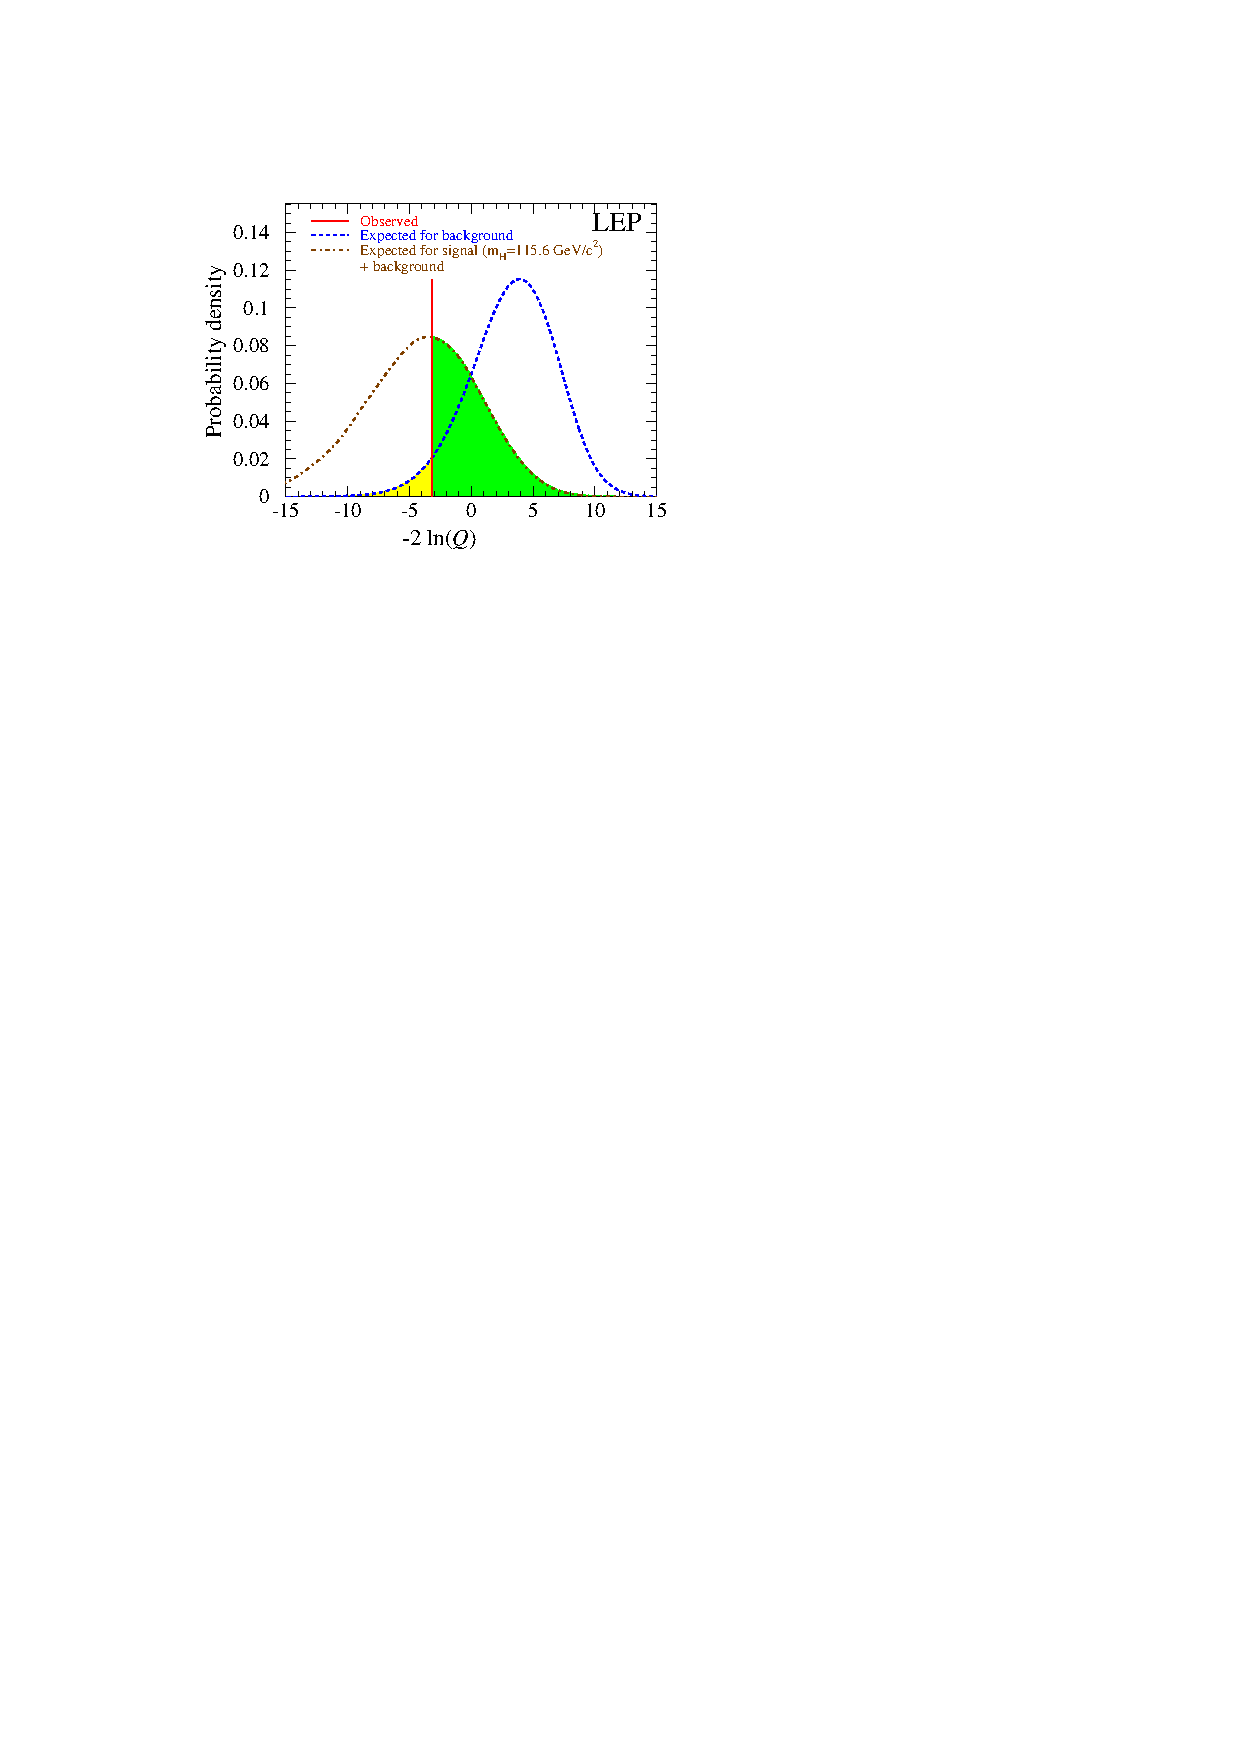
\includegraphics[width=0.95\textwidth]{figures/g21013-fig1.pdf}
\caption{Comparison of the observed value (red line) to the probability densities for $H_{0}$ (background only, blue line) and $H_{1}$ (signal + background, brown line) as a function of the log likelihood ratio. Green area: $\text{CL}_{s+b}$, yellow area: $1-\text{CL}_{b}$. From \cite{Read:presentation}.}
\label{fig:q}
\end{center}
\end{figure}

To set a mass limit on the signal hypothesis, the calculation of $\text{CL}_{s}$ is repeated for different signal masses. Masses with $\text{CL}_{s} < 1 - \alpha$ are excluded at the $\alpha$ confidence level, typically 95\%.
% input: [displays.tex]
\chapter{Event Displays
\label{ch:displays}}
% input: [datasets.tex]
\chapter{Table of Monte Carlo Datasets
\label{ch:datasets}}
% input: [collaboration.tex]
\chapter{CMS Collaboration
\label{ch:collaboration}}

\renewcommand{\baselinestretch}{1}
%\begin{singlespace}
\newpage
\normalsize
\phantomsection
%*input: [mainthesis.bbl]
\providecommand{\href}[2]{#2}\begingroup\raggedright\begin{thebibliography}{10}%
\makeatletter
\providecommand{\hrefCMSnoop }[0]{\@secondoftwo}%
\makeatother
\providecommand{\doi}{\texttt{doi:}\begingroup \urlstyle{tt}\Url}

\bibitem{LHCmachine}
\hrefCMSnoop {} {L.~Evans and P.~Bryant, ``{LHC Machine}'',} \textit{ JINST}
  \textbf{ 3} (2008) S08001,
\href{http://dx.doi.org/10.1088/1748-0221/3/08/S08001}{\doi{10.1088/1748-0221/3/08/S08001}}.
%%CITATION = JINST,3,S08001;%%.

\bibitem{CMSJINST}
\hrefCMSnoop {} {{ CMS} Collaboration, ``{The CMS experiment at the CERN
  LHC}'',} \textit{ JINST} \textbf{ 3} (2008) S08004,
\href{http://dx.doi.org/10.1088/1748-0221/3/08/S08004}{\doi{10.1088/1748-0221/3/08/S08004}}.
%%CITATION = JINST,3,S08004;%%.

\bibitem{Jean-Luc:841573}
\hrefCMSnoop {} {J.-L. Caron, ``{LHC Layout}'',} (September, 1997). AC
  Collection. Legacy of AC. Pictures from 1992 to 2002.

\bibitem{Jean-Luc:841568}
\hrefCMSnoop {} {J.-L. Caron, ``{The LHC injection complex}'',} (May, 1993). AC
  Collection. Legacy of AC. Pictures from 1992 to 2002.

\bibitem{Dailler:842253}
\hrefCMSnoop {} {S.~Dailler, ``{LHC Dipole}'',} (July, 1998). AC Collection.
  Legacy of AC. Pictures from 1992 to 2002.

\bibitem{LumiPublic}
\href {https://twiki.cern.ch/twiki/bin/view/CMSPublic/LumiPublicResults} {{
  CMS} Collaboration, ``{Public CMS Luminosity Information}'',} (Jan, 2014).

\bibitem{Veszpremi:2014hpa}
\hrefCMSnoop {} {{ CMS} Collaboration, ``{Operation and performance of the CMS
  tracker}'',} \textit{ JINST} \textbf{ 9} (2014) C03005,
  \href{http://dx.doi.org/10.1088/1748-0221/9/03/C03005}{\doi{10.1088/1748-0221/9/03/C03005}},
\href{http://www.arXiv.org/abs/1402.0675}{\texttt{ arXiv:1402.0675}}.
%%CITATION = ARXIV:1402.0675;%%.

\bibitem{CMS:2013ecal}
\href {https://cds.cern.ch/record/1528235} {{ CMS} Collaboration, ``{2012 ECAL
  detector performance plots}'',} CMS Detector Performance Summary
  CMS-DP-2013-007, CERN, 2013.

\bibitem{Brooke:2013hnf}
\hrefCMSnoop {} {{ CMS} Collaboration, ``{Performance of the CMS Level-1
  Trigger}'',} \textit{ PoS} \textbf{ ICHEP2012} (2013) 508,
\href{http://www.arXiv.org/abs/1302.2469}{\texttt{ arXiv:1302.2469}}.
%%CITATION = ARXIV:1302.2469;%%.

\bibitem{Trocino:2014jya}
\hrefCMSnoop {} {D.~Trocino, ``{The CMS High Level Trigger}'',} \textit{ J.
  Phys. Conf.} \textbf{ 513} (2014) 012036,
\href{http://dx.doi.org/10.1088/1742-6596/513/1/012036}{\doi{10.1088/1742-6596/513/1/012036}}.
%%CITATION = 00462,513,012036;%%.

\bibitem{CMS-PAS-LUM-12-001}
\hrefCMSnoop {} {{ CMS} Collaboration, ``{CMS Luminosity Based on Pixel Cluster
  Counting - Summer 2012 Update}'',} CMS Physics Analysis Summary
  CMS-PAS-LUM-12-001, CERN, Geneva, 2012.

\bibitem{CMS-PAS-LUM-13-001}
\hrefCMSnoop {} {{ CMS} Collaboration, ``{CMS Luminosity Based on Pixel Cluster
  Counting - Summer 2013 Update}'',} CMS Physics Analysis Summary
  CMS-PAS-LUM-13-001, CERN, Geneva, 2013.

\bibitem{Read:CLs}
\href {http://cdsweb.cern.ch/record/451614} {A.~L. Read, ``Modified frequentist
  analysis of search results (the CLs method)'',} {CERN} Report
  CERN-OPEN-2000-005, 2000.

\bibitem{Read:presentation}
\hrefCMSnoop {} {A.~L. Read, ``{Presentation of search results: the $CL_{s}$
  technique}'',} \textit{ J. Phys. G} \textbf{ 28} (2002) 2693,
  \href{http://dx.doi.org/10.1088/0954-3899/28/10/313}{\doi{10.1088/0954-3899/28/10/313}}.

\end{thebibliography}\endgroup
%FLATEX-REM:\bibliographystyle{lucas_unsrt} 
%FLATEX-REM:\bibliography{mybib}
%\end{singlespace}

\end{document}
